\documentclass[a4paper,14pt, openany, twoside, draft]{extbook} % computer modern font calls
% При завершении (верстке) заменить draft на final!!!!
\usepackage[final]{graphicx}
\graphicspath{{./img/}} % Местонахождение картинок
\usepackage[usenames]{xcolor}
\usepackage{siunitx}
\usepackage{supertabular}
\usepackage{tabulary}
% \usepackage[final]{minted} % Удобный пакет для представления программного кода, требует внешнюю программу и специальные параметры запуска. В отличие от пакета listings поддерживаются русские буквы и utf-8.
%\usemintedstyle{emacs} % Разные стили цвета текста
%\usemintedstyle{tango}
%\usemintedstyle{trac} % better (more bold faces}
%\usemintedstyle{manni} % pastel colors
%\usemintedstyle{bw}    % Черно-белый стиль, следует использовать при верстке печатных документов

%\setminted{breaklines=true,fontsize=\small,funcnamehighlighting=true,python3=true} % Настройка параметров пакета minted

%\newminted{prolog}
%\protect\newminted[proexp]{prolog}{style=bw} % Создание специального окружения для кода языка Prolog.  Окружение позволяет не расцвечивать примеры-запросы.

% Main style definition
% ---------------------
% ISU standard handbook.
%\usepackage[times,fancybot,firamono]{subook} % looks less good than inconsolata
\usepackage[times,fancybot,inconsolata,cambriamath,irnitu]{subook} % Собственно загрузка стиля.
%\usepackage[fancybot,inconsolata,cambriamath]{subook} % Собственно загрузка стиля.
%\usepackage[times]{subook}

% Заменить в коде кой-что на математические формулы
% http://www.tug.org/texlive/Contents/live/texmf-dist/doc/latex/base/alltt.pdf

% Требования к оформлению Типографии ИГУ
% http://lawinstitut.ru/ru/about/services/izdatelstvo/trebovaniya.html
%

% ISU standard monograph (less restrictive and more artistic)
% Из этого примера можно взять настройки стиля для нашего стиля ;-).
% mag не надо использовать! Он тут чисто исторически остался.
% \usepackage[monograph,mag,times,smalltitles,fancybot,listbib,ptfonts,microtyping]{subook}

% Some artistism for monograph
% ----------------------------
%\makeatletter{}
%\renewcommand\su@chapter@font{\sffamily\sfcpshape\bfseries}
%\renewcommand\su@chapter@font@size{\LARGE}
%\makeatother{}
%\floatname{algorithm}{Процедура}
%\renewcommand{\listalgorithmname}{Список процедур}
%\renewcommand\cftsecnumwidth{5ex}
%\tolerance=5000
%\renewcommand{\chaptername}{Глава}
%\usepackage[final]{hyperref}

\newcommand{\AAA}{\textup{\AA}}
\newcommand{\vect}[1]{\mathbf{#1}}

\definecolor{mygreen}{rgb}{0,0.6,0} % Цвета для отображения комментариев.
\definecolor{mygray}{rgb}{0.5,0.5,0.5}
\definecolor{mymauve}{rgb}{0.58,0,0.82}


\usepackage{tikz}  % Очень мощный пакет для рисования, но и одновременно очень сложный.
\usetikzlibrary{arrows,arrows.meta,shapes} % Библиотеки для пакета.
\usetikzlibrary{shadows}
\newcommand*\keystroke[1]{% Команда используется для отображения нажатий клавиш.
  \tikz[baseline=(key.base)]
    \node[%
      draw,
      fill=white,
      drop shadow={shadow xshift=0.25ex,shadow yshift=-0.25ex,fill=black,opacity=0.75},
      rectangle,
      rounded corners=4pt,
      inner sep=1pt,
      line width=0.7pt,
      font=\footnotesize\sffamily
    ](key) {~#1~\strut}%
  ;%
}

\long\def\rem#1{} % Используется для комментирования больших кусков текста.
\def\emphbib#1{#1} % Заглушка для оформления стилей заголовков книг в списке литературы
%\newenvironment{questions}{\subsubsection*{Вопросы для самопроверки}\begin{enumerate}\itemsep0pt minus 0.3pt\parskip0pt plus 0.3pt}{\end{enumerate}}

%\newtheorem{example}{Пример}[chapter]
\hypersetup{
    bookmarks=true,         % show bookmarks bar?
    unicode=true,           % non-Latin characters in Acrobat’s bookmarks
    pdftoolbar=true,        % show Acrobat’s toolbar?
    pdfmenubar=true,        % show Acrobat’s menu?
    pdffitwindow=false,     % window fit to page when opened
    pdfstartview={FitH},    % fits the width of the page to the window
    pdftitle={Название работы},    % title
    pdfauthor={Автор},     % author
    pdfsubject={О чем идет речь в работе},   % subject of the document
    pdfcreator={EMACS-24.5:AuCTeX},   % creator of the document
    pdfproducer={LuaLaTeX}, % producer of the document
    pdfkeywords={Ключевое слово 1} {Ключевое слово 2} {Ключевое слово 3}, % list of keywords
    pdfnewwindow=true,      % links in new window
    colorlinks=true,       % false: boxed links; true: colored links
    linkcolor=[rgb]{0 0.4 0.1},          % color of internal links (black)
    citecolor=blue,        % color of links to bibliography
    filecolor=black,      % color of file links
    urlcolor=[rgb]{0.3 0.0 0.3}           % color of external links
}

%\renewcommand{\headrulewidth}{1pt}

\clubpenalty=3000
\widowpenalty=3000
%\brokenpenalty=10000
%\floatingpenalty=10000

%% \setdefaultlanguage{russian}
%% \setmainlanguage{russian}
%% \setotherlanguage{english}

%\newenvironment{mygroup}{}{}

%\renewcommand\baselinestretch{1.5} % Для диплома.

\definecolor{rclr}{rgb}{0.5,0.1,0.1}
\definecolor{eclr}{rgb}{0,0.5,0.5}
\colorlet{acolor}{blue}
\colorlet{rcolor}{red}
\definecolor{ncolor}{rgb}{0.5,0.5,0.1}
\newcommand{\aaa}[2][acolor]{\noindent\textcolor{eclr}% Использую для пометки места, где надо текста добавить
{+\ [}\textcolor{#1}{#2}\textcolor{eclr}{]}}
\newcommand{\rrr}[2][rcolor]{\noindent% Использую для пометки места, где текста надо убрать
\textcolor{eclr}{-\ [}\textcolor{#1}{#2}\textcolor{eclr}{]}}
\newcommand{\nnn}[2][ncolor]{\noindent% Использую для пометки места, где надо на что-то обратить внимание
\textcolor{eclr}{!\ [}\textcolor{#1}{#2}\textcolor{eclr}{]}}
%\newcommand{\goforth}[1]{$\,\hookrightarrow$\pageref{#1}} % Фича для рисования знака быстрого перехода через раздел, если нет его смысла читать.

% \begin{figure} % Шаблон для включения .pdf_latex - файлов, генерируемых редактором Inkscape
%   \centering
%   \def\svgwidth{\columnwidth}
%   \includesvg{image}
% \end{figure}

%Настройка ниже поджимает абзацы друг к другу, но визуально никак не заметно (пока).
\parskip=0pt plus 0.3pt
\begin{document}
% \itemsep3pt plus 0pt minus 3pt
% \widowpenalty=10000
% \clubpenalty=10000
% \renewcommand\sutitlefontface{\Large\ptsans\nwshape\bfseries}
% \theorembodyfont{\rmfamily}

%\renewcommand{\chaptername}{} % for ISU Handbooks
\renewcommand{\refname}{Список использованных источников} % ... also
\renewcommand{\bibname}{\refname}
\begin{titlepage}
\thispagestyle{empty}
%\aaa{Эта и следующая страница вставляется из .docx}
\begin{center}{\small{}
Министерство образования и науки
Российской Федерации\\
Федеральное государственное бюджетное образовательное\\
учреждение высшего профессионального образования\\
<<Иркутский национальный исследовательский технический университет>> \\[1ex]
Федеральное государственное бюджетное учреждение науки \\
<<Институт геохимии им.~А.~П.~Виноградова
Сибирского отделения РАН>> \\[1ex]
Федеральное государственное бюджетное учреждение науки \\
<<Институт земной коры Сибирского отделения РАН>>
}
\vfill
\hbox to \linewidth{\hfill\bfseries А.~Л.~Финкельштейн, Т.~Ю.~Черкашина\hfill}
 \vspace{2em}
{\large\bfseries Учебное пособие}\\
\vspace{1em}
{Учебное пособие}
\vfill
%\vfill
\vfill
 \textbf{Иркутск 2015}
\end{center}
\end{titlepage}

\clearpage
%\setcounter{page}{2}
\tableofcontents
\clearpage

\chapter{Введение}
\label{cha:intro}

\section{Историческая справка}
\label{sec:history}

[http://nuclphys.sinp.msu.ru/introduction/nobelprice.html] \\\relax
[http://physchem.chimfak.rsu.ru/Source/history/Persones/Roentgen.html]

РЁНТГЕН Вильгельм Конрад, (Wilhelm Conrad Röntgen)

\begin{figure}
\centering
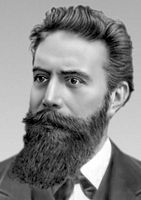
\includegraphics[width=4.794cm,height=6.798cm]{a11-img001.jpg}
\end{figure}
27 марта 1845 г.~-- 10 февраля 1923~г. Первая Нобелевская премия по физике, 1901~г.

Немецкий физик Вильгельм Конрад Рёнтген родился в Леннепе, небольшом городке в Пруссии, и был единственным ребенком в семье торговца Фридриха Конрада Рёнтгена и Шарлотты Констанцы (в девичестве Фровейн) Рёнтген.

Рёнтген поступил в Утрехтскую техническую школу в 1862 году, но был исключен за то, что отказался назвать своего товарища, нарисовавшего непочтительную карикатуру на нелюбимого преподавателя.  Не имея официального свидетельства об окончании школы, он не мог поступить в Утрехтский университет, но стал вольнослушателем.

1865~г. был зачислен студентом в Федеральный технологический институт в Цюрихе и в 1868 году получил диплом.  Август Кундт, известный немецкий физик, обратил внимание на блестящие способности Рёнтгена и посоветовал ему заняться физикой.  Тот последовал его совету и через год защитил докторскую диссертацию в Цюрихском университете.   До 1872~г. Рёнтген работал в физических лабораториях университетов Вюрцбурга, Страсбурга, Гисена и снова Вюрцбурга под руководством физика-экспериментатора А.~Кундта, потом самостоятельно.

8 ноября 1895~г. профессор университета баварского города Вюрцбурга Вильгельм Конрад Рёнтген впервые наблюдал неизвестные ранее лучи, проникающие через непрозрачные преграды.  27 ноября того же года шведский изобретатель и промышленник Альфред Бернхард Нобель (1833–1896) подписал в Париже завещание.  Этим судьбоносным событиям довелось встретиться через пять лет.

Английский физик Уильям Крукс обнаружил, что стенки стеклянной трубки (трубка Крукса), из которой был откачан воздух с помощью усовершенствованного вакуумного насоса, и в которой вызывали высоковольтный разряд между электродами, флуоресцируют зеленоватым светом.  Крукс показал, что лучи испускает отрицательный электрод (помещенный внутрь трубки крестообразный предмет отбрасывал тень на противоположную стенку), и что лучи состоят из некоторой субстанции и несут отрицательный электрический заряд.  Ударяясь о лопасти легкого колесика, лучи приводили его во вращение, а пучок лучей отклонялся магнитом в сторону, соответствующую отрицательному заряду.  В 1878~г. Крукс высказал гипотезу о том, что флуоресценцию вызывают лучи, когда ударяются о стеклянные стенки.  Так как отрицательный электрод называется катодом, испускаемое стенками излучение получило название \emph{катодных лучей}.

Рёнтген повторил некоторые из более ранних экспериментов, в частности показав, что исходящие катодные лучи (тогда еще неизвестные) вызывают флуоресценцию экрана, покрытого цианоплатинитом бария.  Однажды, 8 ноября 1895~г., Рёнтген, чтобы облегчить наблюдения, затемнил комнату и обернул трубку Крукса плотной непрозрачной черной бумагой.  К своему удивлению, он увидел на стоявшем неподалеку экране, покрытом цианоплатинитом бария, полосу флуоресценции.  Тщательнейшим образом проанализировав и устранив возможные причины ошибок, он установил, что флуоресценция появлялась всякий раз, когда он включал трубку, что источником излучения является именно трубка, а не какая-нибудь другая часть цепи и экран флуоресцировал даже на расстоянии почти двух метров от трубки, что намного превосходило возможности короткодействующих катодных лучей.

Следующие семь недель он провел, исследуя явление, которое он назвал \emph{икс-лучами} (т.~е. неизвестными лучами).  Тень, которую отбрасывал на флуоресцирующий экран проводник от индукционной катушки, создававшей необходимое для разряда высокое напряжение, навела Рёнтгена на мысль об исследовании проникающей способности икс-лучей в различных материалах.  Рёнтген заметил, что свинец непроницаем для икс-лучей и сделал поразительное открытие: кости его руки отбрасывали на экран более темную тень, окруженную более светлой тенью от мягких тканей.  Вскоре он обнаружил, что икс-лучи вызывают не только свечение экрана, покрытого цианоплатинитом бария, но и потемнение фотопластинок (после проявления) в тех местах, где икс-лучи попадают на фотоэмульсию.  Так Рёнтген стал первым в мире радиологом.  В честь него икс-лучи стали называть \emph{рентгеновскими лучами}.

\begin{figure}
\centering
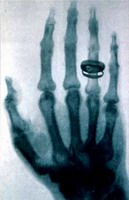
\includegraphics[width=5.546cm,height=8.599cm]{a11-img002.jpg}
\end{figure}
Широкую известность приобрела выполненная Рёнтгеном в рентгеновских лучах фотография (рентгенограмма) кисти руки.  На ней отчетливо видны кости (более плотная костная ткань задерживает икс-лучи, не давая им попасть на фотопластинку) на фоне изображения мягких тканей, задерживающих икс-лучи в меньшей степени, и полоски от колец на пальцах.

После открытия Рёнтгена немецкий физик Макс фон Лауэ высказал блестящее предположение о том, что волновой характер рентгеновского излучения можно было бы доказать, используя в качестве дифракционной решетки регулярно расположенные атомы в кристалле.  В 1913~г. эксперимент, предложенный фон Лауэ, был поставлен Вальтером Фридрихом и Паулем Книппингом. Так, открыв неизвестное ранее излучение, Рёнтген внес существенный вклад в ту революцию в физике, которая происходила в начале XX~в.

Значение открытия Рентгена подтверждается присуждением еще нескольких нобелевских премий за работы в области рентгеновских лучей:

– 1914~г., Мах фон Лауэ, за открытие дифракции рентгеновских лучей.\\
– 1915~г., Уильям Генри и Уильям Лоренс Брэгг, за изучение структуры кристаллов с помощью рентгеновских лучей.\\
– 1917~г., Чарльз Баркла, за открытие характеристического рентгеновского излучения.\\
– 1924~г., Карл Зигбан, за исследования спектров в диапазоне рентгеновских лучей.\\
– 1927~г., Артур Комптон, за открытие эффекта рассеяния рентгеновских лучей на свободных электронах вещества.\\
– 1936~г., Петер Дебай, за вклад в изучение молекулярных структур с помощью дифракции рентгеновских лучей и электронов.\\
– 1979~г., А.~Кормак и Г.~Хаунсфилд, за разработку метода осевой (рентгеновской) томографии.\\

Наиболее заметные открытия, связанные с применением X-лучей

{}- в 1922~г. Нобелевская премия присуждена Нильсу Бору за разработку теории периодической системы элементов, используя закономерности изменения рентгеновских спектров;

{}- в 1922~г. А.~Довийе открыл элемент Гафний по рентгеновским спектрам;

{}- в 1925~г. cупруги Вальтер и Ида Т.~Ноддак открыли элемент Рений по рентгеновским спектрам;

{}- в 1946~г. Нобелевская премия по физиологии и медицине присуждена Герману Меллеру за обнаружение и изучение мутаций под действием рентгеновских лучей;

{}- в 1962~г. Нобелевская премия по химии присуждена Джону К.~Кендрю~и Максу Ф.~Перуц за установление структуры глобулярных белков методом рентгеноструктурного анализа;

{}- в 1964~г. Нобелевским лауреатом по химии стала женщина~-- англичанка Дороти Кроуфут-Ходжкин: методом рентгено-структурного анализа она определила строение белков и ряда биологически активных соединений;

{}- в 1981~г. Кай Сигбан (сын Карла Сигбана) удостоился Нобелевской премии по физике за разработку рентгеновской электронной спектроскопии~-- метода широко применяемого в химических исследованиях;

{}- 1988~г. Нобелевскую премию по химии получили Иоганн Дайзенхофер, Хартмут Михель и~Роберт Хубер за установление трёхмерной структуры фотосинтетического реакционного центра;

{}- в 2002~г. Нобелевская премия по физике присуждена Р.~Джаккони за вклад в астрофизику, который привел к открытию рентгеновских космических источников.

В России уже в январе 1896~г. А.С.~Попов в Кронштадте получил рентгеновские снимки для публичных демонстраций.  В письме В.~Рёнтгену профессор И.И.~Боргман 3~(15) февраля 1896~г. сообщал результаты экспериментов с Х-лучами, выполненных им совместно с А.Л.~Гершуном.  В приложении к книге с переводом сообщения об открытии Х-~лучей был приведен снимок рентгенограммы и утверждалось, что «отпечаток при помощи лучей Рёнтгена был получен в Физической лаборатории Петербургского университета 12~января, первый снимок руки сделан был 16~января».  Вклад в исследование рентгеновских лучей в России, в первые годы после открытия Рёнтгена, внесли и другие русские исследователи: П.Н.~Лебедев, Б.Б.~Голицын, О.Д.~Хвольсон, Ю.В.~Вульф, А.Ф.~Иоффе и др.   Н.Г.~Егоров организовал первую в России рентгеновскую лабораторию, а А.С.~Попов~-- первый рентгеновский кабинет в Кронштадтском госпитале. В 1897 г. газеты писали, что студент Военно-медицинской академии Н.В.~Вихрев сконструировал прибор, с помощью которого можно было делать одновременно два рентгеновских снимка с двух разных точек. Совмещая оба снимка, исследователь получал объемное изображение.

Под руководством А.С.~Попова рентгеновскими аппаратами были оборудованы крупные корабли российского флота. Так, на крейсере «Аврора» во время Цусимского сражения были рентгенологически обследованы около 40 раненых матросов, что избавило их от мучительных поисков осколков с помощью зонда.

%Применение
%Дефектоскопия.
%Рентгеноспектральный анализ (по первичным спектрам, в том числе микрозондовый, по флуоресцентным спектрам, в том числе рентгенорадиометрия,
%по спектрам поглощения), рентгеноструктурный анализ, рентгеновская микроскопия, рентгеновская сепарация и др.).
%Медицина
%медицинская томография

\section{Рентгеновское излучение}
\label{sec:spectrumtype}

Рентгеновские лучи представляют собой электромагнитное излучение в области энергии приблизительно от 0.1 до 150-300 кэВ или в области длин волн приблизительно от 10\textsuperscript{-2} до 10\textsuperscript{2}~\AAA~(1~\AAA~(ангстрем) = 10\textsuperscript{-8} см = 0.1 нм).

На рисунке ниже отмечена область рентгеновского излучения ({X}-rays) в шкале электромагнитных волн.
%[https:////ru.wikipedia.org/wiki/Файл:EM_spectrum.svg].

\begin{figure}
\centering
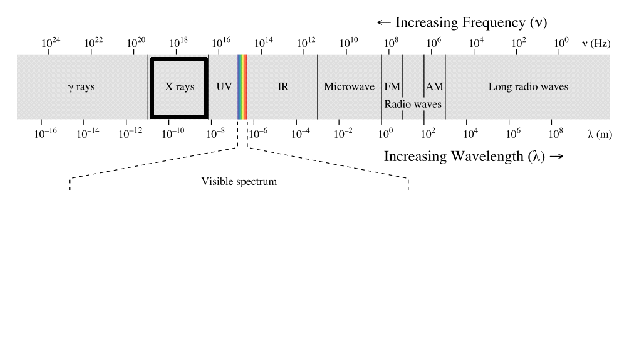
\includegraphics[width=16.595cm,height=7.114cm]{a12-img001.png}
\end{figure}
Энергия электромагнитного излучения $E_{\nu}$  связана с длиной волны ${\lambda}$ и частотой электромагнитной волны ${\nu}$ соотношением
\begin{equation}
\label{eq:energyrad}
%\label{eq:1.1}
E_{\nu }=\mathit{\hslash \nu}=\frac{\hslash c}{\lambda},
\end{equation}
где $\hslash$~-- постоянная Планка, $c$~-- скорость света.
\begin{equation}
\label{eq:energyrad1}
%\label{eq:1.2}
\mathit{E}{\text{(кэВ)}}=\frac{12.398}{\lambda{\text{(ангстрем)}}}.
\end{equation}

\emph{\textbf{Непрерывный и дискретный спектр излучения}}

Два главных процесса обуславливают возникновение рентгеновского излучения.  Рентгеновское излучение образуется в результате ионизации внутренних электронных оболочек атомов заряженными частицами или фотонами, и в результате торможения (потери энергии) электронов или других заряженных частиц в поле атомного ядра и атомных электронов.

\emph{Характеристическое излучение} возникает вследствие электронных переходов между дискретными уровнями атома.  В результате удаления электрона с внутренней оболочки атома вакансия заполняется электронами другой оболочки.  Возникает излучение, энергия которого равна разности энергий уровней атома.  На рисунке ниже приведена схема вероятных переходов между уровнями атома.  Два конкурирующих процесса наблюдаются при возникновении вакансии на внутренней оболочке~-- флуоресценция и оже-эффект.  Эффект Оже более вероятен для низких атомных номеров, в то время как рентгеновское флуоресцентное излучение более вероятно для высоких атомных номеров.

\begin{flushleft}
\tablefirsthead{}
\tablehead{}
\tabletail{}
\tablelasttail{}
\begin{supertabular}{|m{6.866cm}|m{8.0130005cm}|}
\hline
{\selectlanguage{russian} [Warning: Draw object ignored]} &
{\selectlanguage{russian} [Warning: Draw object ignored]}\\\hline
{\selectlanguage{russian} Флуоресценция.  После взаимодействия фотона достаточной энергии с атомом и возникновения вакансии в ${K}$-оболочке она заполняется электроном с ${L}$-оболочки.  Атом покидает рентгеновский фотон характеристической $K_{\alpha}$-линии и фотоэлектрон.} &
{\selectlanguage{russian} Эффект Оже.  После возникновения вакансии в $K$-оболочке она заполняется электроном с $L$-оболочки.  Возникает фотон, энергия которого достаточна для ионизации уровня в $M$-оболочке.  Атом покидает Оже-электрон.}\\\hline
\end{supertabular}
\end{flushleft}
Каждый элемент имеет характеристические K, L и М-серии.  Легкие элементы имеют только K-линии, элементы среднего  диапазона атомных номеров могут испускать и K и L- спектры, в то время как тяжелые элементы имеют K, L и М- спектры.  На рисунке приведена диаграмма основных рентгеновских переходов K, L и М- серий и фрагмент спектра $K$-серии Sr, на котором видны группы $K_{\alpha}$- и $K_{\beta}$- линий.  Индексами ${\alpha}$, ${\beta}$, ${\gamma}$ обозначаются линии в порядке убывания интенсивности.

\begin{flushleft}
\tablefirsthead{}
\tablehead{}
\tabletail{}
\tablelasttail{}
\begin{supertabular}{|m{8.0130005cm}|m{8.485001cm}|}
\hline
{\selectlanguage{russian} [Warning: Draw object ignored] 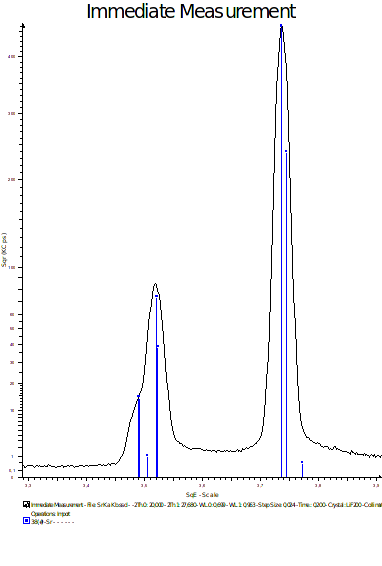
\includegraphics[width=7.44cm,height=11.128cm]{a12-img002.png} } &
{\selectlanguage{russian}  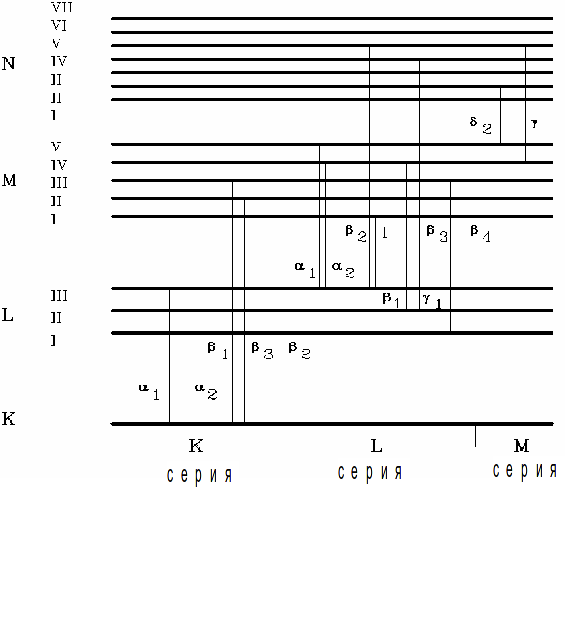
\includegraphics[width=8.285cm,height=9.442cm]{a12-img003.png} }\\\hline
\end{supertabular}
\end{flushleft}
\emph{Тормозное рентгеновское излучение} образуется в результате торможения электронов (или других заряженных частиц) в поле ядра атомов материала анода, имеет непрерывный спектр в области длин волн больше коротковолновой границы  $\lambda_0$, которая определяется ускоряющим электроны напряжением $V$.  Интенсивность тормозного спектра увеличивается с атомным номером материала анода.

На рисунке интенсивность непрерывного спектра дана при трех различных напряжениях для одного и того же материала анода.

 $\lambda _0(\overset{\circ }{A})=\frac{12.398}{V({\text{\textcyrillic{кВ}}})}$ 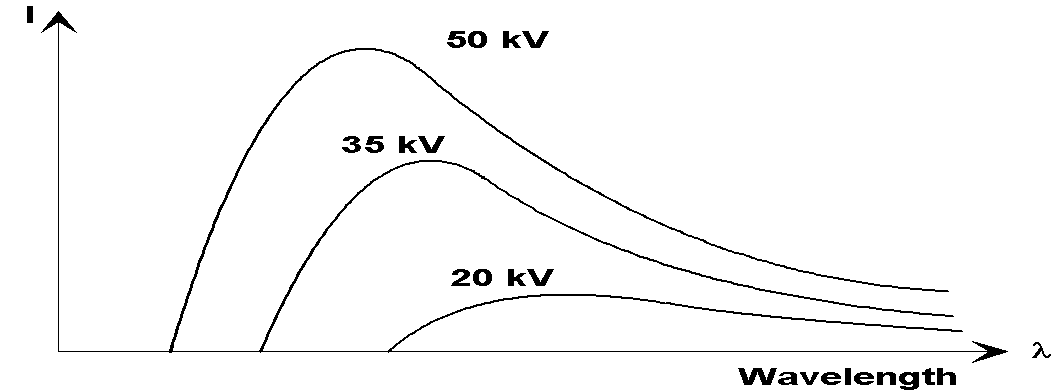
\includegraphics[width=9.049cm,height=5.348cm]{a12-img004.png}

На рисунке ниже в общих чертах изображен спектр рентгеновской трубки с $Rh$-анодом.  На фоне непрерывного тормозного спектра присутствуют характеристические линии $K$- и $L$-~серий Rh.

 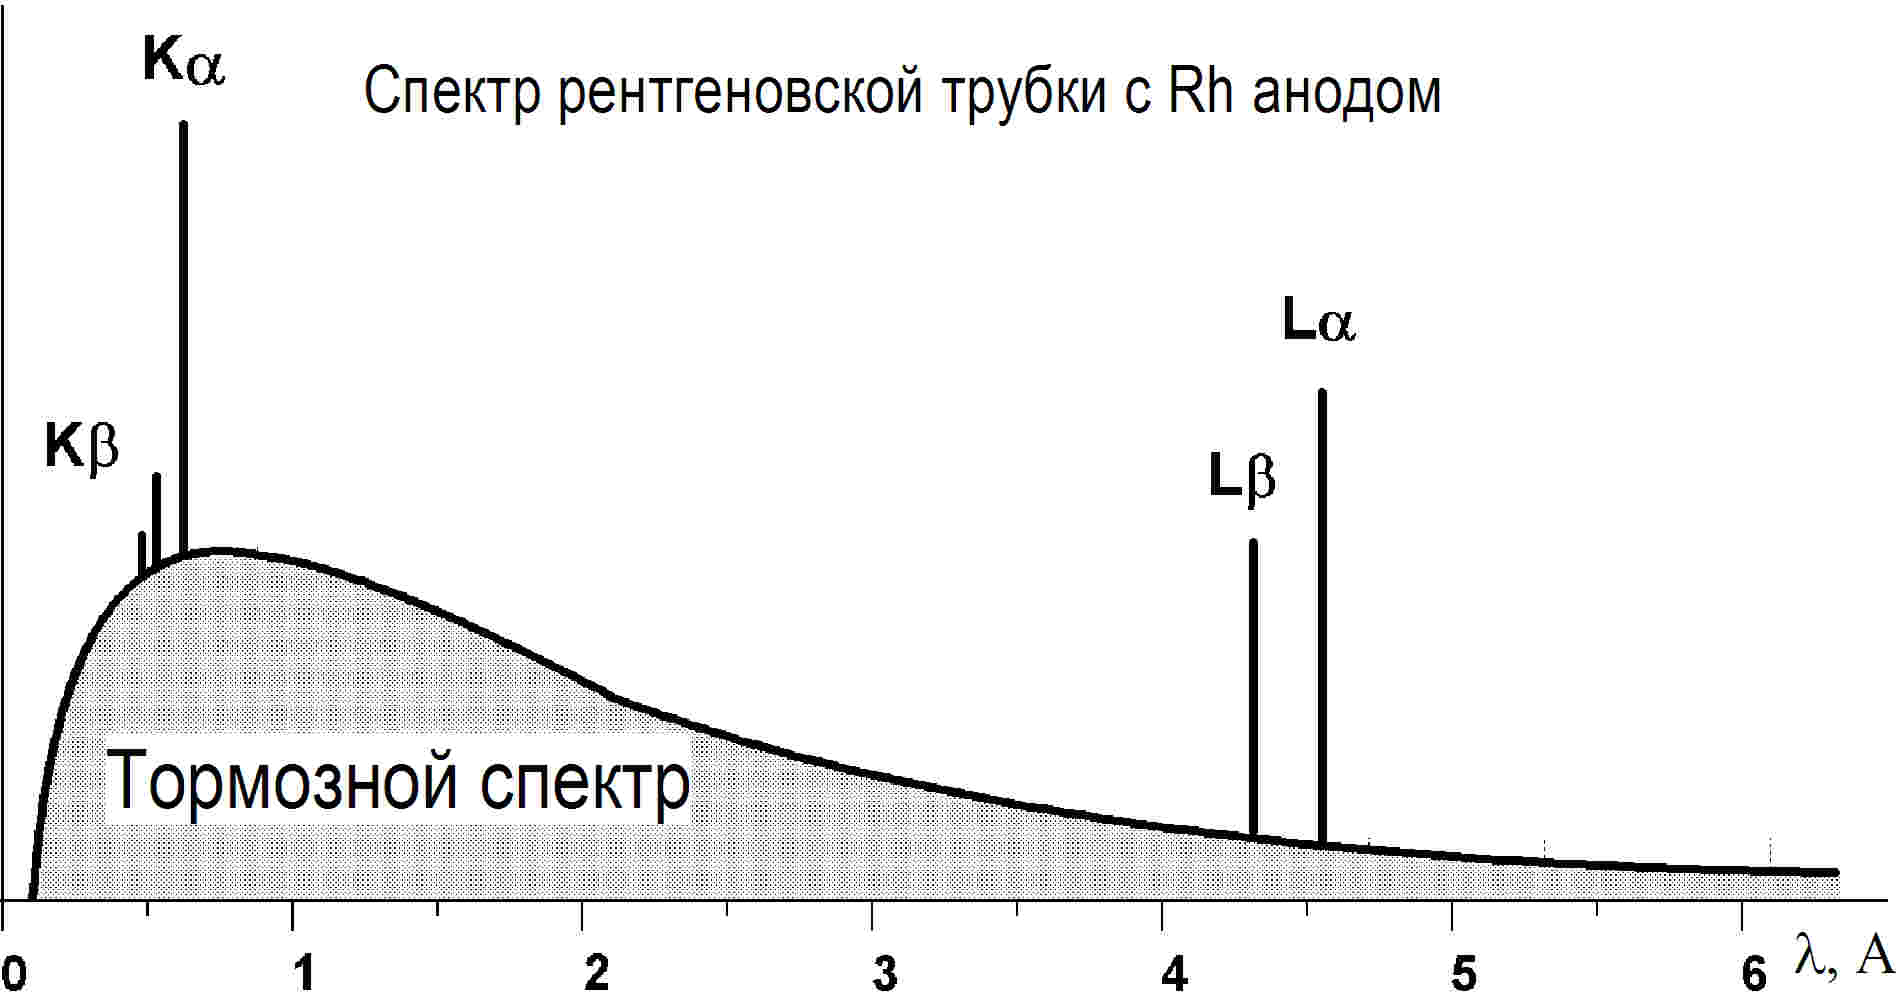
\includegraphics[width=14.944cm,height=7.92cm]{a12-img005.jpg}

\chapter{Модели атома}
\label{cha:model}

\section{Модель атома Бора}
\label{sec:bormodel}

[Зоммерфельд А. Строение атома и спектры. Т. 1. М.: ГИТИ. 1956. Гл. 2. С. 80.]

В модели атома Бора электроны вращаются вокруг ядра по круговым (или эллиптическим орбитам).  Орбита электрона определяется двумя условиями: \emph{классическое и квантовое}.

\emph{Классическое} условие определяет равновесие между центробежной силой и силой кулоновского притяжения
\begin{equation}
\label{eq:energyrad1}
%\label{eq:2.1}
ma\omega^2=\frac{Ze^2}{a^2}\quad\text{или}\quad ma^3\omega^2=Ze^2,
\end{equation}
где $m$~-- масса электрона, $a$ и ${\omega}$~-- радиус орбиты и угловая скорость обращающегося электрона, $e$~-- заряд электрона, $Ze$~-- заряд ядра атома.  Угловая скорость электрона и его скорость  вдоль траектории $\nu$ определены выражением для центробежной силы
\begin{equation}
\label{eq:speedelectron}
%\label{eq:2.2}
\frac{mv^2}{a}=mv\omega=ma\omega^2.
\end{equation}
Квантовое условие накладывается на момент количества движения вращающегося электрона
\begin{equation}
\label{eq:quantcondition}
%\label{eq:2.3}
2\mathit{\pi p}=nh.
\end{equation}
Момент количества движения равен
\begin{equation}
\label{eq:moment}
%\label{eq:2.4}
p=mva=ma^2\omega.
\end{equation}
И, таким образом, квантовое условие имеет вид
\begin{equation}
\label{eq:quantcondition1}
%\label{eq:2.5}
ma^2\omega =\frac{nh}{2\pi}.
\end{equation}
Делением соотношения (\ref{eq:energyrad1}) на (\ref{eq:moment}) получим:
\begin{equation}
\label{eq:nu}
%\label{eq:2.6}
\nu=\mathit{a\omega}=\frac{2\pi Ze^2}{nh},
\end{equation}
\begin{equation}
\label{eq:omega}
%\label{eq:2.7}
a=\frac{n^2h^2}{4\pi^2mZe^2},\quad\omega=\frac{n^2h^2}{4\pi^2mZe^2}.
\end{equation}
В случае атома водорода ($Z=1$) и радиус первой боровской орбиты ($n=1$) равен
\begin{equation}
\label{eq:radius}
%\label{eq:2.8}
a_0=\frac{h^2}{4\pi^2me^2}=5.29\cdot\text{10\textsuperscript{-9} см = 0.529\,\AAA}.
\end{equation}
Далее введем величину $\alpha=\frac{v_0}{c}$, где $v_0$~-- скорость электрона водородного атома на первой боровской орбите, $с$~-- скорость света.  Согласно (\ref{eq:nu}) имеем
\begin{equation}
\label{eq:alpha1}
%\label{eq:2.9}
\alpha=\frac{v_0}{c}=\frac{2\mathit{\pi e^2}}{hc}= 1/137.
\end{equation}
Величина $\alpha$~-- постоянная тонкой структуры~-- имеет существенное значение при рассмотрении электромагнитного взаимодействия.

Полная энергия равна сумме кинетической и потенциальной энергии $W=E_{\text{кин}}+E_{\text{пот}}$.
\begin{equation}
\label{eq:energykinet}
%\label{eq:2.10}
E_{\text{кин}}=\frac{mv^2}{2}=\frac{2\pi^2mZ^2e^4}{n^2h^2},
\end{equation}
\begin{equation}
\label{eq:energypot}
%\label{eq:2.11}
E_{\text{пот}}=-\frac{Ze^2}{a}=-\frac{4\pi^2mZ^2e^4}{n^2h^2}
\end{equation}
И, таким образом, получим
\begin{equation}
\label{eq:fullenergy}
%\label{eq:2.12}
W_n=-\frac{2\pi^2mZ^2e^4}{n^2h^2}.
\end{equation}

\begin{figure}
\centering
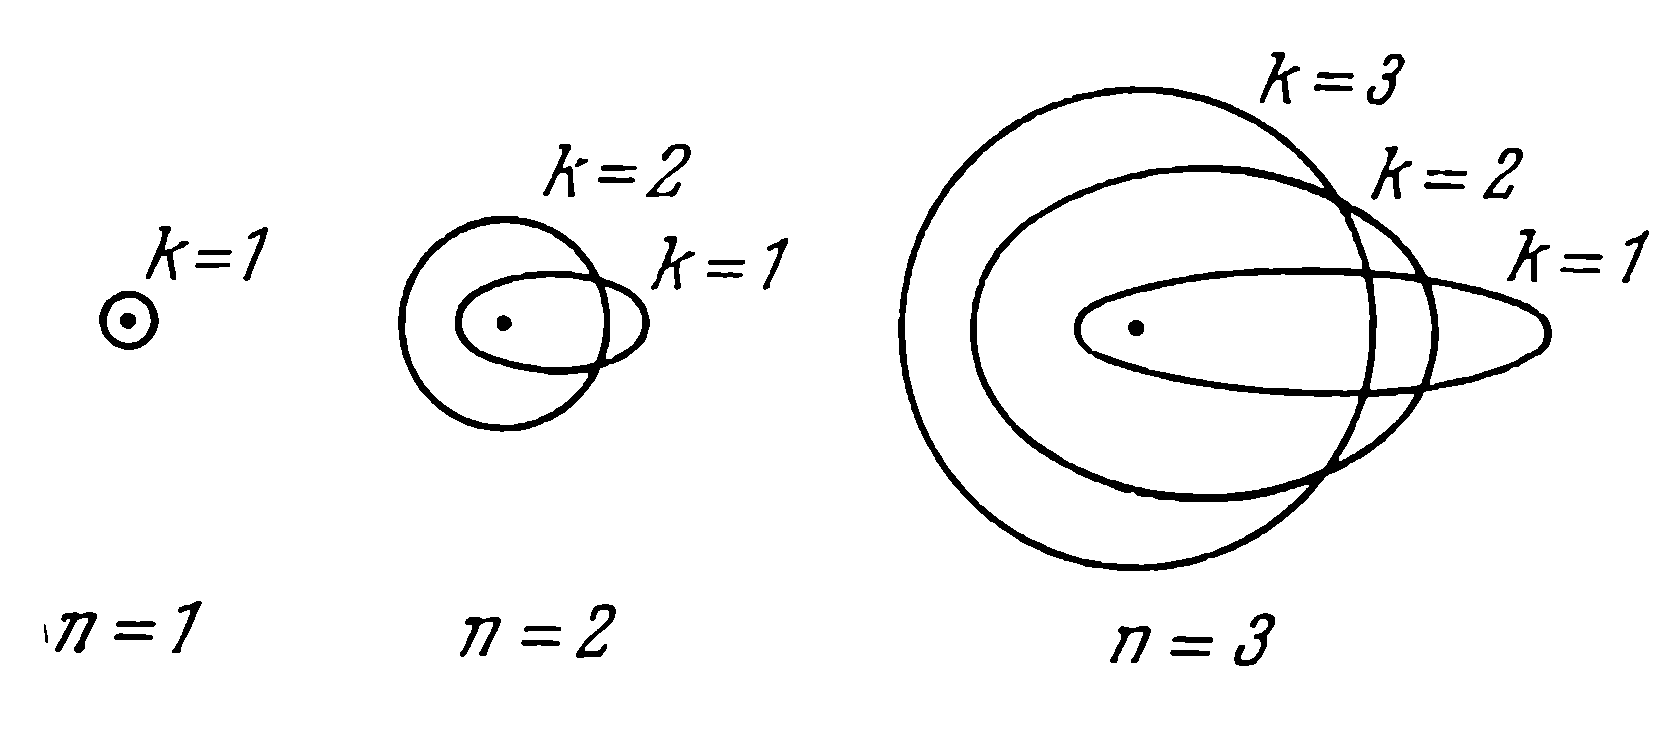
\includegraphics[width=7.091cm,height=3.157cm]{a21-img001.png}
\end{figure}
В модели Бора также возможны эллиптические орбиты той же энергии.  Для каждой энергии имеется $n$ возможных орбит с моментами импульса:
$L=kh/2\pi$,\quad k=1, 2, 3, …, n~ ($k\leq n$).

При $k=n$ орбита является круговой, другие орбиты~-- эллипсы.

Совокупность орбит с определенным $n$ называют \emph{оболочками}.  Оболочку $n=1$ называют $K$-оболочкой, оболочку $n=2$~-- $L$-оболочкой, и т.д.  $M$-, $N$-, $O$-~оболочки.

Энергия излучения  $E_{\gamma }$ будет равна разности энергий уровней (оболочек), между которыми происходит переход электрона
\begin{equation}
\label{eq:energyradiation}
%\label{eq:2.13}
E_{\gamma }=hv=W_n-W_m,
\end{equation}
\begin{equation}
\label{eq:energyradiation1}
%\label{eq:2.14}
E_{\gamma }=RhcZ^2(\frac {1}{n^2}-\frac {1}{m^2}),\quad v=RZ^2(\frac {1}{n^2}-\frac {1}{m^2}),
\end{equation}
где введена постоянная Ридберга $R=\frac{2\pi^2me^4}{ch^3}$.

Выражение (\ref{eq:energypot}) с хорошей точностью позволяет оценить энергии некоторых линий характеристического рентгеновского излучения, например, $K_{\alpha}$-линий.  Следует только учесть, что на $K$-оболочке $(n=1)$ в соответствии с принципом Паули находится два электрона и электрон, находящийся на $L$-оболочке $(n=2)$ находится в поле ядра, экранированного оставшимся на $K$-оболочке электроном, т.~е. для перехода $L\rightarrow K$ вместо $Ze$ следует взять эффективное значение $(Z-1)e$.  Тогда
\begin{equation}
\label{eq:energyradiation2}
%\label{eq:2.15}
E_{\gamma }=13.6\,{\mathit{\text{эВ}}}\cdot(Z-1)^2(\frac{1}{n^2}-\frac{1}{m^2}),
\end{equation}
где постоянная величина в формуле (\ref{eq:energyradiation1}) $Rhc=13.6$ выражена в единицах \text{эВ}.

Из выражения (\ref{eq:energyradiation2}) для излучения $K_{\alpha1}$-линии Na находим $E_{\gamma}=1020\,\text{эВ}$.  Точное измеренное значение энергии излучения $NaK_{\alpha1}$-линии равно 1040.98 эВ.

Для излучения $L$-серии, когда электрон переходит с $M$-оболочки $(n=3)$ на $L$-оболочку $(n=2)$, он чувствует ядро, экранированное оставшимися 9-ю электронами на $K$- и $L$~-оболочках.  Следует ожидать, что эффективный заряд будет равен $(Z-9)e$.  В действительности экранирование будет несколько меньше.  Для учета этого эффекта вводят постоянную экранирования ${\sigma}$, т.~е. эффективный заряд будет равен $(Z-{\sigma})e$.

Так для излучения $L_{\alpha}$-линии молибдена, $(Z=42)$, и $\sigma\approx 7$, и
\begin{equation*}
\label{eq:energyradiation3}
E_{\gamma}=13.6\,{\text{эВ}}\cdot(Z-\sigma)^2(\frac {1}{n^2}-\frac {1}{m^2})=13.6\,{\text{эВ}}\cdot(42-7)^2(\frac {1}{2^2}-\frac {1}{4^2}) = 2301 \text{эВ}.
\end{equation*}
Измеренное значение энергии излучения $MoL_{\alpha}$-линии равно 2292 эВ.

Таким образом, довольно простая полуклассическая теория Бора позволила с удивительной точностью оценивать энергии характеристических линий рентгеновского спектра.

Из выражения (\ref{eq:energyradiation1}) непосредственно следует эмпирический закон Мозли
\begin{equation*}
\sqrt {\nu}\sim Z,
\end{equation*}
где $\nu$~-- частота электромагнитных волн характеристических линий рентгеновского спектра.

\section{Статистическая модель атома Томаса-Ферми}
\label{sec:statmodel}

[Левич В.Г., Вдовин Ю.А., Мямлин В.А. Курс теоретической физики. Т. 2. М.: Наука. 1971. Гл. 11. С. 285.]

Для тяжелых многоэлектрнных атомов получил применение метод Томаса-Ферми, в котором предполагается, что взаимодействие между электронами является достаточно слабым и электроны атома можно рассматривать как идеальный ферми-газ при абсолютном нуле температуры.

В вырожденном ферми-газе электроны попарно заполняют квантовые состояния, так что на каждую пару приходится ячейка фазового пространства объемом ($2\pi \hslash$).  При этом в пространстве импульсов заполнены все ячейки с импульсом в интервале  $0\le p\le p_{\text{max}}$.  Значение $p_{max}$ можно выразить через плотность электронного газа $n$ (среднее число электронов в единице объема)
\begin{equation*}
\label{eq:impuls}
dn=\frac{8\pi}{(2\pi \hslash)^3}\,p^2dp.
\end{equation*}
Интегрируя от $p=0$ до $р=p_{max}$ получим
\begin{equation*}
\label{eq:impuls2}
p_{max}^3=\frac{3}{8\pi}(2\pi \hslash)^3\,n.
\end{equation*}
Плотность заряда ${\rho}=en$
\begin{equation*}
\label{eq:density}
\rho =\frac{8\pi e}{3(2\pi \hslash)^3}\,p_{max}^3
\end{equation*}
$p_{max}$ может быть связан с потенциалом $\varphi (r)$ с помощью следующего рассуждения.  Энергия электрона $E$, связанного в атоме, всегда не положительна, т.~е.
\begin{equation*}
\label{eq:elektronenergy}
E=\frac{p^2}{2m}+\mathit{e\varphi} (r)\le 0.
\end{equation*}
Полагаем, что потенциал $\varphi (r)$ вне атома обращается в нуль, откуда для максимального импульса, при $E=0$, находим
\begin{equation*}
\label{eq:maximpuls}
p_{max}=\sqrt{-2me\varphi (r)}.
\end{equation*}
Поэтому плотность электронного заряда связана с потенциалом соотношением
\begin{equation*}
\label{eq:density1}
\rho=\frac{8\mathit{\pi e}}{3(2\pi \hslash)^3}\left(\sqrt{-2me\varphi (r)}\right)^3.
\end{equation*}
Для сферически симметричного потенциала электростатического поля можно записать уравнение Пуассона
\begin{equation*}
\label{eq:puasson}
\Delta \varphi=-4\pi \rho,
\end{equation*}
или
\begin{equation*}
\label{eq:puasson1}
\frac{1}{r^2}\frac{d^2(\mathit{r\varphi})}{dr^2}=\frac{4e}{3\pi \hslash^3}\left(\sqrt{-2me\varphi (r)}\right)^3.
\end{equation*}
Граничные условия для нейтрального атома следующие.  Потенциал должен обращаться в нуль на больших расстояниях, т.~е. $\varphi \rightarrow 0$ при $r\rightarrow \infty$.  Вблизи ядра поле чисто кулоновское
\begin{equation*}
\label{eq:kulonfield}
\varphi (r)\rightarrow \frac{Ze}{r}\quad\text{при}\quad r\rightarrow 0.
\end{equation*}
Для получения решения переходят к безразмерным величинам
\begin{equation*}
\label{eq:kulonfield}
\chi=\frac{\mathit{r\varphi}}{Ze},\quad x=\frac{r}{d},
\end{equation*}
где $e$~-- модуль заряда, $d$~-- постоянная величина с размерностью длины.

Полагая $d$ равным
\begin{equation*}
\label{eq:kulonfield}
d=\frac 1 2\left(\frac{9\pi ^2}{16}\right)^{1/3}\frac{\hbar ^2}{{\text{me}}^2}\frac 1{Z^{1/3}}=0.88\frac{a_0}{Z^{1/3}},
\end{equation*}
где a0 – радиус первой боровской орбиты,

для ${\chi}$  приходим к уравнению

 $\frac{d^2\chi }{{\text{dx}}^2}=\frac{\chi ^{3/2}}{\sqrt x}$,

при граничных условиях

 $\chi \rightarrow 1$ при  $x\rightarrow 0$,

 $\chi \rightarrow 0$ при  $x\rightarrow \propto ?$.

Границы применимости метода Томаса-Ферми связаны с границами применимости квазиклассического приближения, т. е.  $r\text{{\textgreater}{\textgreater}}a/Z$. На больших расстояниях r\~{}a квазиклассическое приближение снова становится неприемлемым, т.е.  $a/Z\text{{\textless}{\textless}}r\text{{\textless}{\textless}}a$. Следствием модели Томаса-Ферми является оценка размера нейтрального атома. В сфере радиусом приблизительно равным  $R=1.33{\text{aZ}}^{1/3}$ заключена половина полного электронного заряда.

Плотность электронов в атоме связана с потенциалом и функцией  $\chi $

 $\rho (r)=\frac{8\mathit{\pi e}}{3(2\pi \hbar )^3}\left(\sqrt{-2{\text{me}}\varphi (r)}\right)^3$= $\left(32Z^2/9\pi \right)^2\left[\frac{\chi (x)} x\right]^{3/2}$.

Плотность электронов определяет амплитуду рассеяния рентгеновских лучей на атомах

 $f=F^2(q)$,  $\hbar q=2\lambda ^{-1}\text{sin}(\vartheta /2)$, где ${\lambda}$,  $\vartheta $ - длина волны излучения и угол рассеяния.

 $F(q)=4\pi \int \rho (r)\frac{\text{sin}({\text{qr}})}{{\text{qr}}}r^2{\text{dr}}$.\ \ \ \

\section{Уравнение Шредингера для атома водорода}
\label{sec:schredinger}
[P. Кристи и  А. Питти. Строение вещества: введение в современную физику. «Наука». 1969. С. 392.]
Атом водорода образует простейшую атомную систему, состоящую из положительно заряженного ядра, называемого протоном, и обращающегося вокруг него единственного отрицательно заряженного электрона.  Так как масса протона в 1836 раз больше массы электрона, можно пренебречь движением ядра и рассматривать электрон, движущийся в кулоновском поле ядра.  Потенциальная энергия электрона в кулоновском поле ядра равна
\begin{equation}
  \label{eq:potenergy}
V(r)=-Ze^2/r,
\end{equation}
где $Ze$~-- заряд ядра (для водорода, конечно, $Z=1$).   Рассмотрим случай $Z>1$, так как результат будет представлять интерес при обсуждении более тяжелых элементов.  Стационарное уравнение Шредингера для электрона, движущегося в поле ядра, имеет вид
\begin{equation}
  %\label{eq:shred1}
 \label{eq:2.16}
\left[-\frac{\hslash^2}{2m}\nabla^2+V(r)\right]\psi (r)=\mathit{E\psi}(r).
\end{equation}
Или в сферических координатах
\begin{equation}
 % \label{eq:shred2}
 \label{eq:2.17}
-\frac{\hslash^2}{2m}\;\frac{1}{r^2}\;\frac{\partial}{\partial r}\;r^2\;\frac{\partial \psi}{\partial r}+\frac{1}{2mr^2}\;{\mathbf{L}}^2\psi-\frac{Ze^2}{r}\;\psi=E\psi,
\end{equation}
где $\mathbf{L}^2=-\hslash^2\left[\frac {1}{\text{sin}\theta}\frac{\partial}{\partial \theta }\text{sin}\theta \frac{\partial}{\partial \theta}+\frac {1}{\text{sin}^2\theta}\frac{\partial^2}{\partial \varphi^2}\right]$~-- оператор момента импульса.  Если волновая функция $\psi$ соответствует состоянию с определенным моментом импульса, то согласно уравнению полного момента импульса $L^2=L_{l}^2=l(l+1)\;\hslash^2$ будем иметь
\begin{equation}
  %\label{eq:impuls}
 \label{eq:2.18}
{\vect{L}}^2\psi=l(l+1)\hslash^2\psi.
\end{equation}
Волновая функция $\psi(r, \theta, \phi)$ может быть представлена в виде произведения функции, зависящей от r и функции, зависящей от угловых переменных
\begin{equation}
 % \label{eq:impuls}
 \label{eq:2.19}
\psi (r, \theta, \phi)=R(r)\,Y(\theta, \phi).
\end{equation}
В результате получается уравнение
\begin{equation}
 % \label{eq:shred3}
 \label{eq:2.20}
-\frac{\hslash^2}{2m}\;\frac{1}{r^2}\;\frac{d}{dr}\;r^2\;\frac{dR}{dr}+
\left[\frac{l(l+1)\hslash^2}{2mr^2}-\frac{Ze^2}{r}\right]R=ER.
\end{equation}

Решения уравнения (\ref{eq:2.20}) с отрицательной энергией, которые удовлетворяют граничным условиям при $r=0$ и $r \rightarrow \infty$, будут давать допустимые энергии электрона в водородоподобном атоме.

Рассмотрим волновые функции при $l=0$.
Определим параметр $\gamma$ через

\begin{equation*}
 \label{eq:gamma}
\gamma\equiv\sqrt{-\frac{2mE}{\hslash}}=\sqrt{\frac{2m|E|}{\hslash}}.
\end{equation*}
В этом случае уравнение Шредингера (\ref{eq:2.20}) запишется в форме
\begin{equation}
\label{eq:shred4}
\frac{d^2R}{dr^2}+\frac{2}{r}\;\frac{dR}{dr}+\frac{2Z}{a_0r}R=\gamma^2R.
\end{equation}
Решение уравнения (\ref{eq:2.20}), удовлетворяющее условию конечности волновой функции при очень больших r, ищется в виде
\begin{equation}
\label{eq:shred5}
R_n=\overset{n-1}{\underset{i=0}{\sum }}C_ir^ie^{-\gamma r},\quad n\geq 1.
\end{equation}
Опуская подробности вычислений, отметим, что условие конечности волновой функции накладывает ограничение для параметра
\begin{equation}
\gamma=\gamma_n=Z/na_0
\end{equation}
и, следовательно, определяет спектр энергии уровней
\begin{equation}
%\label{eq:energyspectrum}
\label{eq:2.21}
E=E_n=-\frac{\hslash^2Z^2}{2ma_0^2n^2}=-\frac{me^4Z^2}{2\hslash^2n^2}=-13.6\frac{Z^2}{n^2}(\textbf{эВ}),
\end{equation}
где $n$~-- любое конечное целое число и $n\geq1$.
Последнее выражение совпадает с выражением для энергии уровней в теории Бора.
Волновая функция основного состояния, $n=1$, будет иметь вид
\begin{equation}
\label{eq:wavefunction}
R_1=C_0e^{-\frac{Zr}{a_0}}.
\end{equation}
Постоянная $C_0$ определяется из условия нормировки
\begin{equation}
\label{eq:wavefunction}
\overset{\infty}{\underset{0}{\int}}4\mathit{\pi r}^2dr|R|^2=1.
\end{equation}
Тогда волновая функция атома водорода в основном состоянии имеет вид
\begin{equation}
%\label{eq:wavefunction H}
\label{eq:2.22}
R_1=\frac {1}{\sqrt{\mathit{\pi a_0^3}}}e^{-\frac{r}{a_0}}.
\end{equation}
И электронная плотность
\begin{equation}
%\label{eq:wavefunction H}
\label{eq:2.23}
\rho (r)=|R|^2=\frac{1}{\mathit{\pi a_0^3}}e^{-\frac{2r}{a_0}}.
\end{equation}
На рисунке ниже приведена зависимость электронной плотности, определяемой волновой функцией атома водорода (сплошная линия), и электронная плотность согласно модели Томаса-Ферми.  Видно различие на малых и больших расстояниях  $r/a_0$. Плотность по Томасу-Ферми медленно спадает при $r/a_0${\textgreater}3-4 и эта область, где нарушается условие применимости модели.

\begin{figure}[hbt]
  \centering
  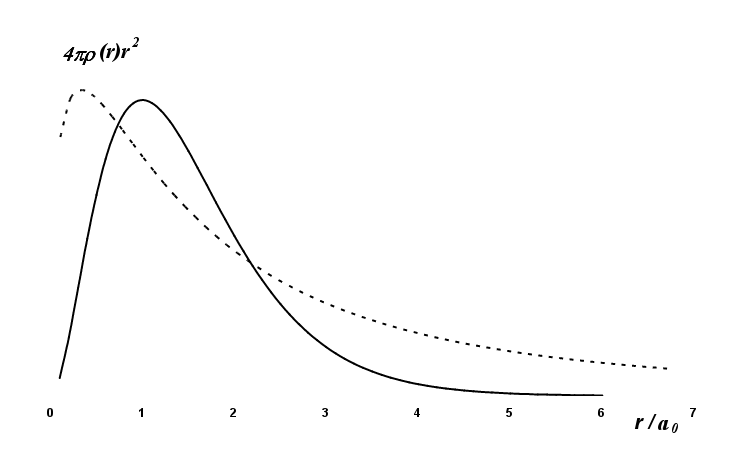
\includegraphics[width=10.421cm,height=6.514cm]{a2324-img001.png}
  \caption{Электронная плотность}
  \label{fig:elecdens}
\end{figure}

В общем случае, волновая функция определяется тремя квантовыми числами ($\mathit{n}$, $\mathit{l}$, $\mathit{m_l}$) в соответствии с тремя координатами  $(r,\theta ,\varphi)$.  $m_l$~-- магнитное квантовое число, которое определяет собственные значения оператора проекции момента импульса $L_z$, зависящего от координаты ${\varphi}$, на выделенное направление ось z
\begin{equation}
\label{eq:operator L}
L_z\psi_m=\frac{\hslash}{i}\frac{\partial}{\partial \varphi}\psi_m=m_l\hslash \psi_m.
\end{equation}
$m_l$~-- может принимать значения от –$l$ до $l$, включая 0, т.~е. $2l+1$ значений.

Энергетические уровни атома водорода зависят только от главного квантового числа $n$, т.е. волновые функции, имеющие одно и то же $n$, но различные азимутальные и магнитные квантовые числа, принадлежат одному энергетическому уровню.  Такая ситуация называется $\emph{\text{вырождением}}$.  Вырожденными являются все уровни атома водорода, кроме наинизшего.

Уравнение Шредингера не учитывает собственный момент электрона ~-- «спин». Собственный момент электрона ~-- спин~-- был установлен Гаудстмитом и Уленбеком (1926 г.) при наблюдении расщепления некоторых спектральных линий и впервые обнаружен в опытах Штерна и Герлаха (1921 г.).  Возможные значения квантового числа собственного момента электрона $m_s$ {}-1/2 и +1/2. Значение спина $s=1/2$.

Для описания состояния электрона в атоме вводят квантовое число, определяющее полный момент импульса системы
\begin{equation}
\label{eq:kvant}
j=l\pm s.
\end{equation}
Полный момент импульса системы складывается из орбитального момента и спина электрона.

В результате учета релятивистских поправок выражение для энергии уровней водородоподобного атома может быть записано в следующем виде [Блохин]
\begin{equation}
%\label{eq:energylevel}
\label{eq:2.24}
E_n=-Rhc\;\frac{M_z}{M_z+m}\left[\frac{Z^2}{n^2}+\alpha^2\frac{Z^4}{n^4}\left(\frac{n}{j+1/2}-\frac{3}{4}\right)\right],
\end{equation}
где $M_z$~-- масса ядра атома с атомным номером $Z$.  Поскольку ${\alpha}$=1/137 малая величина, второй член в квадратных скобках имеет значение для относительно больших Z.

Точное решение уравнение Шредингера найдено только для атома водорода.  Для остальных атомов используют приближенные численные методы решения.  Приближенный метод расчета волновых функций электронов в атомах, получивший широкую известность, был предложен Хартри в 1927 году.  Метод был назван методом самосогласованного поля и заключается в том, что волновая функция атома представляется в виде суперпозиции волновых функций отдельных электронов, которые движутся в самосогласованном поле, создаваемом ядром и всеми остальными электронами.  В этом приближении уравнение Шредингера может быть записано в виде
\begin{equation}
\label{eq:energylevel}
\hat H\psi=\mathit{E\psi},\qquad\hat H=\left[-\frac{\hslash^2}{2m}\overset N{\underset i{\sum }}\nabla_i^2-\overset N{\underset i{\sum }}\frac{Ze^2}{r_i}+\overset N{\underset i{\sum}}\overset N{\underset{j\neq i}{\sum}}\frac{e^2}{|r_i-r_j|}\right].
\end{equation}
В методе Хартри волновая функция атома представляется в виде суперпозиции волновых функций отдельных электронов.  Слэттер предложил искать радиальные одноэлектронные функции в виде
\begin{equation}
\label{eq:energylevel}
\psi_n=A_nr^{n^\ast -1}\text{exp}(-\gamma_n\frac {r}{a_0}),
\end{equation}
где  $n^\ast$~-- эффективное главное квантовое число,\;$\gamma_{n,l}=\frac{Z-\sigma_{n,l}}{n^\ast a_0}$.
Фок добавил в уравнение слагаемое, связанное с так называемым обменным взаимодействием.  Уравнения самосогласованного поля называют уравнениями Хартри-Фока-Слэттера (ХФС, HFS).

\section{Распределение электронов в атомах}
\label{sec:electron-in-athoms}
[Блохин М.А. Физика рентгеновских лучей. М.: ГИТТЛ, 1957. С. 17.]

Значение главного квантового числа $n$ определяет электронную оболочку, к которой относится электрон
\begin{table}[hbt]
\begin{tabular}{rlllllll}
\label{tab:kvant}
$n$~= &1 &2 &3 &4 &5 &6 \\
оболочка: &$K$ &$L$ &$M$ &$N$ &$O$ &$P$ \\
\end{tabular}
\end{table}
Тип состояния определяется значением азимутального квантового числа \\
\begin{table}[hbt]
\begin{tabular}{rlllllll}
\label{tab:azimut}
$l$~= &1 &2 &3 &4 &5 \\
тип: &$s$ &$p$ &$d$ &$f$ &$g$ \\
\end{tabular}
\end{table}
Для данного квантового числа $n$ существует $2l+1$ значений магнитного квантового числа $m$ и два значения спинового квантового числа $m_s=\pm 1/2$.  При заданном $n$ число $l$ может принимать значения 0, 1, …, $n$-1.  Таким образом, полное число различных комбинаций трех квантовых чисел $l$, $m$ и $m_s$ при данном $n$ равно сумме
\begin{equation}
\label{eq:summquant}
\overset {n-1}{\underset{l=0}{\sum}}2(2l+1)=2n^2,
\end{equation}
т.е. 2, 8, 18, 32, …… при $n$~=1, 2, 3, 4,…...
В соответствии с принципом Паули два электрона не могут иметь один и тот же набор квантовых чисел  $n$, $l$, $m$ и $m_s.$ Следовательно, в оболочке с главным квантовым числом n может находить не более $2n^2$ электронов. Распределение электронов по состояниям принято записывать следующим образом: $1s^2$.

Первая цифра дает значение главного квантового числа, буква обозначает тип состояния и азимутальное квантовое число, верхний индекс обозначает число электронов, находящихся в этом состоянии.

В таблице~\ref{tab:spd} приведено распределение электронов в атомах благородных газов.
\begin{table}[hbt]
\caption{Распределение электронов в атомах благородных газов}
 \begin{tabular}{rllllllllllll} \label{tab:spd}
 2 &He &$1s^2$ \\
10 &Ne &$1s^2$ &$2s^2$ &$2p^6$ \\
18 &Ar &$1s^2$ &$2s^2$ &$2p^6$ &$3s^2$ &$3p^6$ &$3d^10$ \\
36 &Kr &$1s^2$ &$2s^2$ &$2p^6$ &$3s^2$ &$3p^6$ &$3d^10$ &$4s^2$ &$4p^6$ &$4d^10$ \\
54 &Xe &$1s^2$ &$2s^2$ &$2p^6$ &$3s^2$ &$3p^6$ &$3d^10$ &$4s^2$ &$4p^6$ &$4d^10$ &$5s^2$ &$5p^6$ \\
 \end{tabular}
\end{table}
Совокупность электронов, занимающих состояния с различными $l$ и $j=l\pm s$ называют \emph{подоболочками} или \emph{подуровнями}.

В таблице~\ref{tab:eledistr} ниже приведено распределение электронов для первых трех оболочек по подуровням и их обозначения.
\begin{table}[hbt]\centering
  \caption{Распределение электронов для первых трех оболочек по подуровням и их обозначения}
  \label{tab:eledistr}
\small
\begin{tabulary}{1.05\textwidth}{|C|C|C|C|L|C|C|C|}
\hline
$n$ & \parbox[t]{1.7cm}{\centering Уровень,\\ оболочка\\[0.3em]} & $l$ & Орбита & \centering $m$ & $j$ & Подоболочка & \parbox[t]{2.8cm}{\centering Число \\ электронов \\ на подуровне} \\
\hline
1 & $K$ & 0 & $s$ & 0 & 1/2 & -- & 2 \\
\hline
2 & $L$ & 0 & $s$ & 0 & 1/2 & $L_I$ & 2 \\
  &     & 1 & $p$ & -1, 0, +1 & 1/2 & $L_{II}$ & 2 \\
  &     &   &     &           & 3/2 & $L_{III}$ & 4 \\
\hline
3 & $M$ & 0 & $s$ & 0 & 1/2 & $M_I$ & 2 \\
  &     & 1 & $p$ & -1, 0, +1 & 1/2 & $M_{II}$ & 2 \\
  &     &   &     &           & 3/2 & $M_{III}$ & 4 \\
  &     & 2 & $d$ & -2, -1, 0, +1, +2 & 3/2 & $M_{IV}$ & 4 \\
  &     &   &     &           & 5/2 & $M_{V}$ & 6 \\
\hline
\end{tabulary}
\end{table}

\chapter{Характеристический рентгеновский спектр}
\label{cha:character}

\section{Энергии рентгеновских уровней атома}
\label{sec:x-levels}

[ Павлинский Г.В.  Основы физики рентгеновского излучения. – М.:ФИЗМАТЛИТ, 2007. с. 15.]

[ Блохин М.А. Физика рентгеновских лучей. М.: ГИТТЛ, 1957. с. 25. ]

Энергии рентгеновских уровней с удаленным электроном во внутренней оболочке атома подобны энергиям уровней водородоподобного атома.

За нулевой рентгеновский уровень энергии принимают энергию атома, из которого удален один электрон.

При переходе электрона с внешнего на внутренний уровень атом совершает переход из состояния с большей энергией в состояние с меньшей энергией, т.е. уменьшает свою энергию.

В соответствии с квантовой механикой, электроны распределены в объеме атома, т.е. электрон на внутренней оболочке в некоторой степени экранируется от ядра другими электронами атома. Поэтому эффективный заряд ядра учитывают c помощью замены Z  на (Z{}-${\sigma}$1) , где ${\sigma}$1 – постоянная полного экранирования. Кроме этого вводят также постоянною внутреннего экранирования ${\sigma}$2 , которая отражает влияние взаимодействия между азимутальным и спиновым моментом в незамкнутой оболочке. Полный момент совокупности электронов, заполняющих некоторую оболочку, равен нулю. После удаления электрона из оболочки она приобретает некоторый момент j.

Таким образом, выражение для энергии рентгеновского уровня атома, полученое из выражения (2.24) для водородоподобного атома, имеет вид

 $E(\normalsubformula{\text{n,l,j}})\normalsubformula{\text{=Rhc}}\frac{M_z}{M_z\normalsubformula{\text{+m}}}\left[\frac{(Z-\sigma _1)^2}{n^2}\normalsubformula{\text{+\textgreek{a}}}^2\frac{(Z-\sigma _2)^4}{n^4}\left(\frac n{\normalsubformula{\text{j+}}1/2}-\frac 3 4\right)\right]$\ \ \ \ \ \ (3.1)

Постоянная ${\sigma}$2 может быть определена из измерения разности энергий так называемых спин-дублетов.

Спин-дублеты - линии рентгеновского спектра, обусловленные переходами с уровней отличающихся только значением спинового квантового числа j=l+1/2 и j=l{}-1/2.

Для  разности энергий линий спин-дублета K${\alpha}$1 и K${\alpha}$2 (переходы с уровня  n=2, l=1, ms -1/2 и +1/2) из выражения (3.1) следует

 $\normalsubformula{\text{\textgreek{D}E=E}}(\normalsubformula{\text{n,l,l+}}1/2)-E(\normalsubformula{\text{n,l,l}}-1/2)\normalsubformula{\text{=Rhc\textgreek{a}}}^2\frac{(Z-\sigma _2)^4}{n^3l(\normalsubformula{\text{l+}}1)}$.\ \ \ \ \ \ \ \ (3.2)

Для элемента железа (Z=26), ${\Delta}$E=12.9эВ. Из выражения (3.2)

\begin{equation*}
\normalsubformula{\text{\textgreek{D}E=}}13.6\normalsubformula{\text{\textcyrillic{эв}}}\left(\frac 1{137}\right)^2\frac{(26-\sigma _2)^4}{2^31(1+1)}
\end{equation*}
находим ${\sigma}$2 =2.9.

${\sigma}$1 может быть определена из закона Мозли. Пренебрегая членом порядка ${\alpha}$2 в выражении (3.1) получим  $\sqrt{E_v}\normalsubformula{\text{=A}}(Z-\sigma _1)$, где А постоянная для выбранной линии спектра. Как уже отмечалось в разделе 2.1 постоянная полного экранирования ${\sigma}$1  для K{}-серии приблизительно равна 1.

В таблице приведены энергии K${\alpha}$1{}-линии (EK${\alpha}$1) нескольких элементов, выбранные из данных [ http://xdb.lbl.gov/Section1/Table\_1-2.pdf ], рассчитанные по формуле (3.1) и по простой формуле (2.5). Видно, что формула (3.1) обеспечивает хорошее согласие с данными  [ http://xdb.lbl.gov ]. Погрешность расчета по формуле (2.15) менее 1\% отн. наблюдается только для Z{\textless}27. С увеличением Z расхождение расчетов по формулам (3.1) и (2.5) увеличивается.

\begin{center}
\tablefirsthead{}
\tablehead{}
\tabletail{}
\tablelasttail{}
\begin{supertabular}{|m{1.6329999cm}|m{1.4929999cm}|m{1.663cm}|m{1.698cm}|}
\hline
\centering{\selectlanguage{russian} Элемент} &
\centering{\selectlanguage{russian} EK${\alpha}$1 , эВ} &
\centering{\selectlanguage{russian} Формула (3.1)} &
\centering\arraybslash{\selectlanguage{russian} Формула (2.15)}\\\hline
\centering{\selectlanguage{russian} 11 Na} &
\centering{\selectlanguage{russian} 1041} &
\centering{\selectlanguage{russian} 1020} &
\centering\arraybslash{\selectlanguage{russian} 1020}\\\hline
\centering{\selectlanguage{russian} 21 Sc} &
\centering{\selectlanguage{russian} 4091} &
\centering{\selectlanguage{russian} 4095} &
\centering\arraybslash{\selectlanguage{russian} 4080}\\\hline
\centering{\selectlanguage{russian} 27 Co} &
\centering{\selectlanguage{russian} 6930} &
\centering{\selectlanguage{russian} 6944} &
\centering\arraybslash{\selectlanguage{russian} 6895}\\\hline
\centering{\selectlanguage{russian} 31 Ga} &
\centering{\selectlanguage{russian} 9252} &
\centering{\selectlanguage{russian} 9272} &
\centering\arraybslash{\selectlanguage{russian} 9180}\\\hline
\centering{\selectlanguage{russian} 41 Nb} &
\centering{\selectlanguage{russian} 16615} &
\centering{\selectlanguage{russian} 16642} &
\centering\arraybslash{\selectlanguage{russian} 16320}\\\hline
\centering{\selectlanguage{russian} 51 Sb} &
\centering{\selectlanguage{russian} 26359} &
\centering{\selectlanguage{russian} 26336} &
\centering\arraybslash{\selectlanguage{russian} 25500}\\\hline
\centering{\selectlanguage{russian} 61 Pm} &
\centering{\selectlanguage{russian} 38725} &
\centering{\selectlanguage{russian} 38525} &
\centering\arraybslash{\selectlanguage{russian} 36720}\\\hline
\centering{\selectlanguage{russian} 71 Lu} &
\centering{\selectlanguage{russian} 54070} &
\centering{\selectlanguage{russian} 53423} &
\centering\arraybslash{\selectlanguage{russian} 49980}\\\hline
\centering{\selectlanguage{russian} 81 Tl} &
\centering{\selectlanguage{russian} 72872} &
\centering{\selectlanguage{russian} 71281} &
\centering\arraybslash{\selectlanguage{russian} 65280}\\\hline
\centering{\selectlanguage{russian} 92 U} &
\centering{\selectlanguage{russian} 98439} &
\centering{\selectlanguage{russian} 94697} &
\centering\arraybslash{\selectlanguage{russian} 84466}\\\hline
\end{supertabular}
\end{center}
Дублеты экранирования. Несмотря на то, что азимутальное квантовое число l не входит в явном виде в формулу (3.1), для уровней энергии атома с одинаковыми числами n и j , но отличающимся значением числа l,  будут отличаться постоянные экранирования ${\sigma}$1  и ${\sigma}$2 , и, следовательно, величины энергии соответствующих уровней. К таким парам уровней относятся (L1 и L2), (M1 и M2), (M3 и M4), (N1 и N2) и т.д. Эти пары уровней получили название «дублеты экранирования». Пара линий рентгеновского спектра, возникающая при переходе с этих уровней на один общий уровень, или пара линий, возникающих при переходе с одного общего уровня на каждый из таких уровней, также называется дублетом экранирования. К таким дублетам можно отнести, например, линии железа K${\beta}$1 (переход KM3) и K${\beta}$5 (переход KM4).

Разность энергий уровней дублета экранирования можно оценить следующим образом. Пренебрегая членом порядка ${\alpha}$2 в выражении (3.1) для двух уровней дублета получим

 $\sqrt E=\sqrt{\normalsubformula{\text{Rhc}}}\frac{(Z-\sigma _1)} n$ и $\sqrt{\normalsubformula{\text{E'}}}=\sqrt{\normalsubformula{\text{Rhc}}}\frac{(Z-\sigma _1')} n$.

Следовательно, в грубом приближении

 $\Delta \sqrt E=\sqrt{\normalsubformula{\text{Rhc}}}\frac{\normalsubformula{\text{\textgreek{Ds}}}_1} n$\ \ \ \ \ \ \ \ \ \ \ \ \ \ \ \ (3.3)

3.2. Диаграмма линий и правила отбора

[ Блохин М.А. Физика рентгеновских лучей. М.: ГИТТЛ, 1957. с. 53. ]

Для обозначения рентгеновских уровней атома используют следующие символы

1s1/2  \ \ 2s1/2  \ \ 2p1/2  \ \ 2p3/2  \ \ 3s1/2  \ \ 3p1/2  \ \ 3p3/2  \ \ 3d3/2  \ \ 3d5/2  \ \ и т.д.

\ \ \ \ K\ \ LI\ \ LII\ \ LIII\ \ MI\ \ MII\ \ MII\ \ MIV\ \ MV \ \ и т.д.

Оболочки с n=4, 5, 6, 7 обозначаются буквами N, O, P, Q.

На рисунке приведена диаграмма переходов, соответствующих основным линиям K{}- и L{}-серии рентгеновского спектра.

 \includegraphics[width=17.154cm,height=10.846cm]{a3-img/a3-img001.jpg}

Группа линий, возникающая в результате переходов на K-оболочку, называется K-серией, группа линий, возникающая в результате переходов на L-оболочку, называется L-серией и т.д. Подробная база данных линий рентгеновского спектра приведена на сайте http://www.nist.gov/pml/data/xraytrans/index.cfm.

На рисунке ниже приведены рентгеновские спектры K- и L-серии стронция, записанные на кристалл-дифракционном спектрометре. В спектре K-серии видны две группы линий K\textlatin{[F061?]} (KL3(K\textlatin{[F061?]}1 ),  KL2~ (K\textlatin{[F061?]}2 )) и K\textlatin{[F062?]} (KM2~(K\textlatin{[F062?]}3), KM3~(K\textlatin{[F062?]}1), KN2,3~(K\textlatin{[F062?]}2~), KM4,5~(K\textlatin{[F062?]}5~)) ,. В спектре L-серии видны три группы линий L\textlatin{[F061?]} (L3M4~(L\textlatin{[F061?]}2), L3M5~(L\textlatin{[F061?]}1)), L\textlatin{[F062?]}1,3 (L1M3~(L\textlatin{[F062?]}3), L2M4~(L\textlatin{[F062?]}1)) и L\textlatin{[F062?]}2,3 (L3N5~(L\textlatin{[F062?]}2), L1M3~(L\textlatin{[F062?]}3)). Разрешающая способность спектрометра недостаточна для разделения всех интенсивных линий, которые помечены маркерами. Слабые \textlatin{[F067?]}-линии на рисунках не видны.

\begin{flushleft}
\tablefirsthead{}
\tablehead{}
\tabletail{}
\tablelasttail{}
\begin{supertabular}{|m{7.7970004cm}|m{7.84cm}|}
\hline
{\centering\selectlanguage{russian} K-серия Sr\par}

\centering{\selectlanguage{russian}  \includegraphics[width=7.056cm,height=10.541cm]{a3-img/a3-img002.png} } &
{\centering\selectlanguage{russian} L{}-серия Sr\par}

\centering\arraybslash{\selectlanguage{russian}  \includegraphics[width=6.874cm,height=10.287cm]{a3-img/a3-img003.png} }\\\hline
\end{supertabular}
\end{flushleft}
Группа наиболее интенсивных линий спектра называется «электрическими дипольными линиями». Эти линии возникают при соблюдении определенных правил для квантовых чисел уровней. Правила отбора для электрических дипольных линий следующие.

1.   $\normalsubformula{\text{\textgreek{D}n}}\neq 0$.\ \ \ \ \ \ \ \ \ \ \ \ \ \

2.   $|\normalsubformula{\text{\textgreek{D}l}}|=1$,\ \  или \ \  $\normalsubformula{\text{\textgreek{D}l}}\text{=+1,}-1$.\ \ \ \ \ \ \ \ \ \ (3.4)

3.   $|\normalsubformula{\text{\textgreek{D}j}}|=\text{0,1}$, или\ \  $\normalsubformula{\text{\textgreek{D}j}}\text{=+1,0,}-1$\ \ \ \ \ \ \ \

Правила отбора для \emph{l} позволяют объяснить, почему, например, отсутствует переход L1→K, а правила отбора для j объясняют, почему маловероятны переходы, для которых  $\normalsubformula{\text{\textgreek{D}j=}}2$.

Кроме электрических дипольных линий, в рентгеновском спектре наблюдаются некоторые очень слабые линии, называемые «электрическими квадрупольными линиями», возникающие при соблюдении следующих правил:

1.   $\normalsubformula{\text{\textgreek{D}n}}\neq 0$.\ \ \ \ \ \ \ \ \ \

2.   $|\normalsubformula{\text{\textgreek{D}l}}|=\text{0,2}$.\ \ \ \ \ \ \ \ \ \ \ \ (3.5)

3.   $|\normalsubformula{\text{\textgreek{D}j}}|=\text{0,1,2}$.\ \ \ \ \ \ \ \

Линии, удовлетворяющие правилам отбора (3.4) и (3.5) называются «диаграммными» линиями.

3.3. Сателлиты линий.

В рентгеновских спектрах наблюдаются также слабые линии, возникновение которых не может быть объяснено вышеуказанными правилами отбора. Такие линии называются сателлитами, и они возникают вблизи более интенсивных диаграммных линий. Например, в спектре K{}-серии некоторых элементов наблюдаются сателлиты, возникающие вследствие образования двух вакансий на K{}- и L{}-оболочке, как это изображено на следующем рисунке.

 \includegraphics[width=7.994cm,height=5.385cm]{a3-img/a3-img004.png}

На рисунке ниже приведен пример спектра K\textgreek{a}1,2{}-линии и группы сателлитов, возникающих в двукратно ионизованном атоме.

\begin{flushleft}
\tablefirsthead{}
\tablehead{}
\tabletail{}
\tablelasttail{}
\begin{supertabular}{m{17.179998cm}}
{\selectlanguage{russian}  \includegraphics[width=14.815cm,height=10.432cm]{a3-img/a3-img005.png} }

{\selectlanguage{russian} M. Torres Deluigi and J. Díaz-Luque (2012). http://www.intechopen.com/books/x{}-ray{}-spectroscopy/analysis{}-of{}-the{}-k{}-satellite{}-lines{}-in{}-x{}-ray{}-emission{}-spectra.}

\\
\end{supertabular}
\end{flushleft}
В рентгеновских спектрах наблюдаются также сателлиты, возникающие в результате переходов с валентных уровней, участвующих в образовании химических соединений, на внутренние уровни атома (K или L). Интенсивность и энергия таких сателлитов зависит от характера химической связи между атомами.

На рисунке ниже приведен пример спектра вблизи K\textgreek{b}{}-линии серы. Видно, что для соединений серы, в которых присутствует кислород, появляется сателлит K${\beta}$’ , который не наблюдается для соединений, не содержащих кислород.

 \includegraphics[width=15.016cm,height=9.573cm]{a3-img/a3-img006.jpg}


\section{Диаграммные линии и правила отбора}
\label{sec:diag-lines}

\section{Сателлиты линий}
\label{sec:sattelit-lines}

\chapter{Ослабление рентгеновского излучения в веществе (закон Бэра)}
\label{cha:}
 [ Блохин М.А. Физика рентгеновских лучей. М.: ГИТТЛ, 1957. с. 147. ]

При прохождении направленного пучка рентгеновских фотонов через вещество интенсивность (или число фотонов) пучка ослабляется вследствие взаимодействия с атомами вещества. Два основных явления определяют ослабление рентгеновского излучения – поглощение ( фотоэффект на внутренних оболочках атома) и рассеяние (когерентное и некогерентное). В области энергий менее 50-100 кэВ преобладает поглощение. Рассмотрим процесс поглощения пучка рентгеновских фотонов, проходящего через тонкий слой вещества толщиной dx в направлении оси x (см. рисунок).

[Warning: Draw object ignored]

Вероятность dP того, что фотон поглотится в слое dx пропорциональна числу атомов в единице объема вещества n (размерность - 1/см3) и поперечному сечению атома  $\sigma $ (см2) при взаимодействии с которым происходит фотоэффект, т.е. поглощение фотона

\section[\ \ \ \ \ \ \ \ \ \ \ \ \ \ \ \ 4.1]{ $\text{dP}=-\mathit{n\sigma }\text{dx}$ \ \ \ \ \ \ \ \ \ \ \ \ \ \ \ \ 4.1}
Знак минус в выражении 4.1 означает, что число фотонов уменьшается. Согласно определению вероятности  $\text{dP}$ равна доле поглощенных фотонов

 $\text{dP}=\frac{\text{dN}} N$,\ \ или \ \  $\frac{\text{dN}} N=-\mathit{n\sigma }\text{dx}$ \ \ \ \ \ \ \ \ \ \ \ \ 4.2

Для слоя вещества толщиной d  после интегрирования получим \ \ \ \

 $\int _{\Box }^{\Box }\frac{\text{dN}} N=-\int _0^d\mathit{n\sigma }\text{dx}$ \ \ \ \ или\ \ \ \  $\text{ln}(\frac N{N_0})=-\mathit{n\sigma d}$.\ \ \ \ \ \ 4.4

\section[Или ]{Или }
 $N=N_0{\cdot}e^{-\mathit{n\sigma }{\cdot}d}$\ \ .\ \ \ \ \ \ \ \ \ \ \ \ 4.5

Для рентгеновских лучей величину  $\mathit{n\sigma }$ обозначают символом ${\mu}$ .

Величина ${\mu}$ называется линейным коэффициентом ослабления и имеет размерность см{}-1 .

 $N=N_0{\cdot}e^{-\mu {\cdot}d}$ \ \ \ \ \ \ \ \ \ \ \ \ \ \ 4.6

Эта формула носит название закон Бугера-Ламберта-Бэра (или Бугера-Бэра).

Величина L=1/${\mu}$  имеет смысл средней длины пробега фотона в веществе. Функция  $f(x)=\mu {\cdot}e^{-\mu {\cdot}x}$ обладает свойствами функции плотности вероятности. Т. е.  $\int _0^{\Box }f(x)\text{dx}=1$ и вероятность того, что случайная величина ${\lambda}$ (пробег фотона) будет меньше некоторой величины x

 $P(\lambda <x)=F(x)=\int _0^xf(x)\text{dx}=?1-e^{-\mathit{\mu x}}$.

\section[Среднее значение \ случайной длины пробега фотона \ .]{Среднее значение  случайной длины пробега фотона   $\bar x=\int _0^{\Box }\text{xf}(x)\text{dx}=\frac 1{\mu }$.}
Число атомов в единице объема может быть выражено через плотность вещества соотношением

 $n=\frac{N_A} A\rho $, \ \ \ \ \ \ \ \ \ \ \ \ \ \ \ \ 4.7

где NA – число Авогадро, A – атомная масса элемента вещества, ${\varrho}${}- плотность вещества.\ \

Тогда   $\mathit{n\sigma }=\frac{N_A} A\rho {\cdot}\sigma $.

Величина  $\mu _m=\frac{N_A} A\sigma $ называется массовым коэффициентом ослабления и имеет размерность см2/г. Закон ослабления в этом случае имеет вид

 $N=N_0{\cdot}e^{-\mu _m\rho {\cdot}d}$ \ \ \ \ \ \ \ \ \ \ \ \ \ \ \ \ 4.8

\section[Массовый коэффициент ослабления сложного вещества определяется суммой]{Массовый коэффициент ослабления сложного вещества определяется суммой}
 $\mu _m=\sum _iC_i{\cdot}\mu _{\text{mi}}$, \ \ \ \ \ \ \ \ \ \ \ \ \ \ 4.9

где Ci и ${\mu}$mi – массовое содержание и массовый коэффициент ослабления элемента i , содержащегося в веществе.

Из выражения 4.8 нетрудно рассчитать толщину слоя вещества, ослабляющего излучение в k раз

 $D(k)=-\frac 1{\mu _m\rho }\text{ln}(\frac N{N_0})=-\frac 1{\mu _m\rho }\text{ln}(\frac 1 k)$ \ \ \ \ \ \ \ \ \ \ \ \ 4.10

В таблице ниже, в качестве примера, приведены массовые коэффициенты ослабления, линейные коэффициенты ослабления, длины свободного пробега и толщина слоя вещества, ослабляющего интенсивность излучения в 10~000 раз.  Например, излучение с энергией 10 кэВ практически полностью поглощается в слое воздуха приблизительно 2 см. Излучение с энергией 150 кэВ поглощается в слое воздуха толщиной приблизительно 560 м и в слое свинца толщиной только 4 мм.

\begin{flushleft}
\tablefirsthead{}
\tablehead{}
\tabletail{}
\tablelasttail{}
\begin{supertabular}{m{2.299cm}|m{2.162cm}|m{2.292cm}|m{2.2059999cm}|m{1.7459999cm}|m{1.134cm}|m{2.391cm}|}
\hline
\multicolumn{1}{|m{2.299cm}|}{\centering{\selectlanguage{russian} Энергия излучения, кэВ}} &
\centering{\selectlanguage{russian} Вещество} &
\centering{\selectlanguage{russian} ${\mu}$m , см2/г} &
{\centering\selectlanguage{russian} Плотность,\par}

\centering{\selectlanguage{russian} г/см3} &
\centering{\selectlanguage{russian} ${\mu}$ , см{}-1} &
\centering{\selectlanguage{russian} L, см} &
\centering\arraybslash{\selectlanguage{russian} D (0.0001),  см}\\\hline
\multicolumn{1}{|m{2.299cm}|}{\centering{\selectlanguage{russian} 10}} &
\centering{\selectlanguage{russian} Воздух} &
\centering{\selectlanguage{russian} 3606} &
\centering{\selectlanguage{russian} 1.21E-03} &
\centering{\selectlanguage{russian} 4.35} &
\centering{\selectlanguage{russian} 0.230} &
\centering\arraybslash{\selectlanguage{russian} 2.120}\\\hline
 &
\centering{\selectlanguage{russian} Железо} &
\centering{\selectlanguage{russian} 171.84} &
\centering{\selectlanguage{russian} 7.8} &
\centering{\selectlanguage{russian} 1340} &
\centering{\selectlanguage{russian} 0.001} &
\centering\arraybslash{\selectlanguage{russian} 0.007}\\\hhline{~------}
 &
\centering{\selectlanguage{russian} Свинец} &
\centering{\selectlanguage{russian} 130.11} &
\centering{\selectlanguage{russian} 11.3} &
\centering{\selectlanguage{russian} 1470} &
\centering{\selectlanguage{russian} 0.001} &
\centering\arraybslash{\selectlanguage{russian} 0.006}\\\hline
\multicolumn{1}{|m{2.299cm}|}{} &
 &
 &
 &
 &
 &
\\\hline
\multicolumn{1}{|m{2.299cm}|}{\centering{\selectlanguage{russian} 50}} &
\centering{\selectlanguage{russian} Воздух} &
\centering{\selectlanguage{russian} 40.270} &
\centering{\selectlanguage{russian} 1.21E-03} &
\centering{\selectlanguage{russian} 0.049} &
\centering{\selectlanguage{russian} 20.6} &
\centering\arraybslash{\selectlanguage{russian} 189.8}\\\hline
 &
\centering{\selectlanguage{russian} Железо} &
\centering{\selectlanguage{russian} 1.958} &
\centering{\selectlanguage{russian} 7.8} &
\centering{\selectlanguage{russian} 15.27} &
\centering{\selectlanguage{russian} 0.065} &
\centering\arraybslash{\selectlanguage{russian} 0.603}\\\hhline{~------}
 &
\centering{\selectlanguage{russian} Свинец} &
\centering{\selectlanguage{russian} 7.988} &
\centering{\selectlanguage{russian} 11.3} &
\centering{\selectlanguage{russian} 90.27} &
\centering{\selectlanguage{russian} 0.011} &
\centering\arraybslash{\selectlanguage{russian} 0.102}\\\hline
\multicolumn{1}{|m{2.299cm}|}{} &
 &
 &
 &
 &
 &
\\\hline
\multicolumn{1}{|m{2.299cm}|}{\centering{\selectlanguage{russian} 150}} &
\centering{\selectlanguage{russian} Воздух} &
\centering{\selectlanguage{russian} 0.136} &
\centering{\selectlanguage{russian} 1.21E-03} &
\centering{\selectlanguage{russian} 1.63E-04} &
\centering{\selectlanguage{russian} 6120} &
\centering\arraybslash{\selectlanguage{russian} 56368}\\\hline
 &
\centering{\selectlanguage{russian} Железо} &
\centering{\selectlanguage{russian} 0.192} &
\centering{\selectlanguage{russian} 7.8} &
\centering{\selectlanguage{russian} 1.50} &
\centering{\selectlanguage{russian} 0.668} &
\centering\arraybslash{\selectlanguage{russian} 6.153}\\\hhline{~------}
 &
\centering{\selectlanguage{russian} Свинец} &
\centering{\selectlanguage{russian} 2.009} &
\centering{\selectlanguage{russian} 11.3} &
\centering{\selectlanguage{russian} 22.70} &
\centering{\selectlanguage{russian} 0.044} &
\centering\arraybslash{\selectlanguage{russian} 0.406}\\\hhline{~------}
\end{supertabular}
\end{flushleft}
Состав воздуха (массовые  \% ): 75.53\% азот, 23.18\% кислород, 1.29\% аргон.

Суммарное поперечное сечение взаимодействия рентгеновского излучения с атомами вещества равно сумме атомного сечения фотоэффекта (photo effect) и когерентного (coherent) и некогерентного (incoherent) рассеяния на атомах (обычно в единицах барн/атом)

 $\sigma _{\text{tot}}=\sigma _{\text{ph}}+\sigma _{\text{coh}}+\sigma _{\text{inc}}$.\ \ \ \ \ \ \ \ \ \ \ \ \ \ \ \ 4.11

Полный массовый коэффициент ослабления равен сумме коэффициентов фотоэлектрического поглощения, обозначаемого буквой ${\tau}$ , и коэффициентов когерентного и некогерентного рассеяния (обычно в единицах см2/г)

 $\mu _m=\tau _m+\sigma _{m,\text{coh}}+\sigma _{m,\text{inc}}$ \ \ \ \ \ \ \ \ \ \ \ \ \ \ 4.12

На рисунке ниже приведен пример зависимости коэффициентов ослабления и рассеяния от энергии излучения для азота. Видно, что в области энергии {\textless}30 кэВ преобладает поглощение. В области энергии излучения более 50 кэВ доминирующим эффектом становится некогерентное рассеяние.

Подробнее зависимость коэффициентов поглощения и рассеяния от энергии излучения и атомного номера элементов будет рассмотрена в последующих разделах.

 \includegraphics[width=13.966cm,height=16.611cm]{a4-img/a4-img001.png}

Данные сайта [ http://physics.nist.gov/PhysRefData/Xcom/html/xcom1.html ].
\chapter{Тормозной и характеристический рентгеновский спектр, возбужденный потоком электронов}
\label{cha:torm-spec}
5. Тормозной и характеристический рентгеновский спектр, возбужденный потоком электронов

Самым распространенным источником рентгеновского излучения являются рентгеновские трубки, в которых рентгеновское излучение возбуждается потоком падающих на металлическую мишень электронов, ускоренных в электрическом поле при напряжении от десятков до первых сотен кВ.

Ускоренные электроны в твердой мишени испытывают упругое рассеяние - изменение траектории движения электрона при незначительной потере энергии, и неупругое рассеяние – потери энергии при незначительном изменении траектории движения. Упругое рассеяние обусловлено главным образом взаимодействием с ядрами атомов, при котором возникает значительное отклонение траектории движения электрона от первоначальной. Неупругое рассеяние возникает главным образом в результате взаимодействия с атомными электронами.

5.1. Потери энергии (торможение) электронов в веществе

Поскольку большинство электронов атомов мишени принадлежит внешним оболочкам атома и энергия их связи (энергия ионизации атома) порядка 10 эВ (для атома водорода 13.6 эВ), а энергия падающих на мишень электронов 10–100 кэВ на несколько порядков больше энергии связи электронов, падающие электроны теряют свою энергию в основном на ионизацию оболочек атома малыми порциями. Поэтому потери энергии падающих электронов воль траектории движения рассматривают в приближении непрерывного замедления. На рисунке приведен пример траектории электрона в мишени и график зависимости энергии электрона (E) от длины пути вдоль траектории движения (s).

Траектория электрона в мишени может быть представлена в виде малых прямолинейных отрезков, в конце которых электрон меняет направление движения или испытывает потери энергии без изменения направления. На рисунке схематично приведена ступенчатая линия, величина ступенек которой соответствует потере энергии при неупругом столкновении, и аппроксимация кривой линией, соответствующей приближению непрерывного замедления.

\begin{flushleft}
\tablefirsthead{}
\tablehead{}
\tabletail{}
\tablelasttail{}
\begin{supertabular}{m{7.4290004cm}m{8.940001cm}}
{\selectlanguage{russian} [Warning: Draw object ignored]} &
{\selectlanguage{russian} [Warning: Draw object ignored]}

{\selectlanguage{russian} E0 и smax – начальная энергия и максимальная длина пробега электрона в мишени. }\\
\end{supertabular}
\end{flushleft}
Для расчета потерь энергии нерелятивистских электронов используют формулу Бете (вариант формулы Бете-Блоха для заряженных частиц)

 $-\frac{\normalsubformula{\text{dE}}}{\normalsubformula{\text{ds}}}=2\normalsubformula{\text{\textgreek{p}e}}^4\left[\rho \frac{N_A} A\right]Z\frac 1 E\text{ln}(\frac{1.166E} J)$ \ \ \ \ \ \ \ \ \ \ \ \ 5.1

где J - средняя энергия ионизации атома.

Величина  $\left[\rho \frac{N_A} A\right]$ - число атомов в единице объема вещества мишени. И, соответственно, величина  $\left[\rho \frac{N_A} A\right]Z$ есть число электронов в единице объема вещества. Величину

 $\normalsubformula{\text{S=}}-\frac 1{\rho }\frac{\normalsubformula{\text{dE}}}{\normalsubformula{\text{ds}}}=-\frac{\normalsubformula{\text{dE}}}{\normalsubformula{\text{d\textgreek{r}s}}}$ \ \ \ \ \ \ \ \ \ \ \ \ \ \ \ \ 5.2

называют тормозной способностью вещества.

В практических расчетах для средней энергии ионизации используется значение

 $J\approx 11.5\cdot Z$ эВ.\ \ \ \ \ \ \ \ \ \ \ \ \ \ 5.2

Экспериментальные данные величины J обнаруживают значительный разброс. Однако это слабо влияет на расчеты тормозной способности, так как значение J входит в логарифмический член, а логарифм – медленно меняющаяся функция аргумента.

Строгий расчет потерь энергии электронов в результате неупругого рассеяния в твердой мишени довольно сложный. Объяснение формулы 5.1 в весьма упрощенных рассуждениях может быть получено следующим образом.

Быстрый электрон падающего пучка со скоростью ve, пролетая вблизи слабо связанного электрона мишени (почти свободного, покоящегося электрона) на расстоянии b (прицельный параметр) сообщает ему импульс  $\vec P$ (см. рисунок).  [Warning: Draw object ignored]Увеличение энергии покоящегося электрона происходит за счёт кинетической энергии падающего. Предполагаем, что отклонением от прямолинейного пути можно пренебречь.

Далее если считать, что взаимодействие существенно только на некотором расстоянии (отрезке пути), равном 2b, то время пролёта  $\normalsubformula{\text{\textgreek{D}t}}\approx \frac{2b}{v_e}$.

Кулоновская сила  $|\overrightarrow F|$ на этом участке равна  $-\frac{e^2}{b^2}$.  Поэтому  $|\vec P|\approx F\normalsubformula{\text{\textgreek{D}t}}\approx \frac{2e^2}{\normalsubformula{\text{bv}}_e}$. Переданная электрону кинетическая энергия  $T_e=\frac{P^2}{2m_e}=\frac{2e^4}{m_eb^2v_e^2}$, т.е. эту энергию (в среднем) и теряет падающая частица.

Чтобы учесть все электроны, с которыми взаимодействует падающий электрон на расстоянии  $b$, рассматривают кольцевой слой  $\normalsubformula{\text{db}}$ и цилиндр единичной длины  $\normalsubformula{\text{dx}}$ ( $2\normalsubformula{\text{\textgreek{p}bdbdx}}$). В объёме цилиндра находится  $2\normalsubformula{\text{\textgreek{p}bdbdx}}\cdot n_e$ электронов ( $n_e$ - электронная плотность, число электронов в единице объема). В результате взаимодействия с ними электрон падающего пучка теряет энергию на единице длинны пути вдоль трека

 $-\frac{\normalsubformula{\text{dE}}}{\normalsubformula{\text{dx}}}=2\normalsubformula{\text{\textgreek{p}bdbdx}}\cdot n_e\frac{2e^4}{m_eb^2v_e^2}=\frac{4\normalsubformula{\text{\textgreek{p}e}}^4n_e}{m_ev_e^2}\frac{\normalsubformula{\text{db}}} b$.\ \ \ \ \ \

Полные потери энергии получаются после интегрирования в интервале от  $b_{\text{min}}$ до  $b_{\text{max}}$. (При интегрировании от 0 до  $\infty $ получается бессмысленный результат – при  $\normalsubformula{\text{b=}}0$ частица тормозится мгновенно, а при  $\normalsubformula{\text{b=}}\infty $ - интеграл расходится).

\begin{equation*}
-\frac{\normalsubformula{\text{dE}}}{\normalsubformula{\text{dx}}}=\frac{4\normalsubformula{\text{\textgreek{p}e}}^4n_e}{m_ev_e^2}\text{ln}\frac{b_{\text{max}}}{b_{\text{min}}}
\end{equation*}
Максимальные потери энергии  $\normalsubformula{\text{\textgreek{D}E}}_{\text{max}}=2m_ev_e^2$ соответствуют минимальному прицельному параметру  $b_{\text{min}}$, а минимальные потери  $\normalsubformula{\text{\textgreek{D}E}}_{\text{min}}\approx J$ соответствуют  $b_{\text{max}}$. И, таким образом, мы приходим к выражению подобному 5.1.

Максимальный траекторный пробег может быть вычислен из выражения 5.1

 $s_{\text{max}}=\overset 0{\underset{E_0}{\int }}\frac{\normalsubformula{\text{dE}}}{(\normalsubformula{\text{dE}}/\normalsubformula{\text{ds}})}$. \ \ \ \ \ \ \ \ \ \ \ \ \ \ \ \ 5.2

Пробег электронов увеличивается с увеличением энергии электронов приблизительно пропорционально квадрату их энергии

\begin{equation*}
s_{\text{max}}\normalsubformula{\text{=const}}\cdot E_0^2
\end{equation*}
В таблице приведены оценки величины максимального траекторного пробега, вычисленные из выражения 5.1 и 5.2 для алюминия, меди и золота для энергии пучка электронов 10, 50 и 100 кэВ. Пробег электронов уменьшается с увеличением атомного номера мишени и составляет величины от долей мкм до нескольких десятков мкм.

\begin{flushleft}
\tablefirsthead{}
\tablehead{}
\tabletail{}
\tablelasttail{}
\begin{supertabular}{|m{1.7279999cm}|m{1.522cm}|m{1.522cm}|m{1.522cm}|m{1.744cm}|}
\hline
\multicolumn{2}{|m{3.45cm}|}{} &
\raggedleft{\selectlanguage{russian} 10 кэВ} &
\raggedleft{\selectlanguage{russian} 50 кэВ} &
\raggedleft\arraybslash{\selectlanguage{russian} 100 кэВ}\\\hline
\centering{\selectlanguage{russian} Элемент} &
\centering{\selectlanguage{russian} ${\varrho}$, г/см3} &
\multicolumn{3}{m{5.188cm}|}{\centering{\selectlanguage{russian} smax , мкм}}\\\hline
{\selectlanguage{russian} Al} &
\raggedleft{\selectlanguage{russian} 2.7} &
\raggedleft{\selectlanguage{russian} 1.29} &
\raggedleft{\selectlanguage{russian} 22.7} &
\raggedleft\arraybslash{\selectlanguage{russian} 80.5}\\\hline
{\selectlanguage{russian} Cu} &
\raggedleft{\selectlanguage{russian} 8.96} &
\raggedleft{\selectlanguage{russian} 0.54} &
\raggedleft{\selectlanguage{russian} 8.7} &
\raggedleft\arraybslash{\selectlanguage{russian} 30.0}\\\hline
{\selectlanguage{russian} Au} &
\raggedleft{\selectlanguage{russian} 19.32} &
\raggedleft{\selectlanguage{russian} 0.39} &
\raggedleft{\selectlanguage{russian} 5.2} &
\raggedleft\arraybslash{\selectlanguage{russian} 17.3}\\\hline

\section{Поперечные сечения возбуждения характеристического и тормозного излучения электронами}
\label{sec:sections}

\section{Потери энергии (торможение) электронов в веществе (формула Бете)}
\section{Рассеяние электронов в веществе}
5.2. Упругое рассеяние электронов в веществе

Рассеяние электронов на ядрах атомов

[ Л.Д.Ландау, Е.М.Лифшиц. Краткий курс теоретической физики. Книга 1. Механика. Электродинамика. М.: Наука. 1969. с. 51.

 Книга 2. Квантовая механика. М.: Наука. 1972. с. 236. ]

Эффективное поперечное сечение рассеяния может быть определено следующим выражением

 $\normalsubformula{\text{d\textgreek{s=}}}\frac{\normalsubformula{\text{dN}}} n$,\ \ \ \ \ \ \ \ \ \ \ \ \ \ \ \ 5.3

где n – плотность потока, т.е. число частиц, проходящих в единицу времени через единицу площади поперечного сечения однородного пучка. dN – число частиц, рассеянных в единицу времени на углы, лежащие в интервале  $\vartheta $ и  $\normalsubformula{\text{\textgreek{j+}d\textgreek{j}}}$. Величина  $\normalsubformula{\text{d\textgreek{s}}}$ имеет размерность площади. Траектория электрона в поле неподвижного ядра с зарядом +Ze представляет собой гиперболу, асимптоты которой соответствуют направлению движения до и после взаимодействия (см. рисунок). Расстояние ${\varrho}$ называют прицельным параметром.

[Warning: Draw object ignored]

При рассеянии электрона в кулоновском поле ядра прицельный параметр ${\varrho}$ связан с углом рассеяния ${\vartheta}$

 $\normalsubformula{\text{\textgreek{r=}}}\frac{\normalsubformula{\text{Ze}}^2}{\normalsubformula{\text{mv}}_{\infty }^2}\normalsubformula{\text{ctg}}\frac{\vartheta } 2$,\ \ \ \ \ \ \ \ \ \ \ \ \ \ \ \ 5.4

где  $v_{\infty }${}- скорость электрона на бесконечном удалении от рассеивающего ядра.

В таком случае рассеиваются в заданный интервал углов между  $\vartheta $ и  $\normalsubformula{\text{\textgreek{j+}d\textgreek{j}}}$ лишь те частицы, которые летят с прицельным параметром в определенном интервале ${\varrho}$ и ${\varrho}$+d${\varrho}$.

Число таких частиц равно произведению \emph{n} на площадь кольца между окружностями с радиусами ${\varrho}$ и ${\varrho}$+d${\varrho}$, т. е.  $\normalsubformula{\text{dN=}}2\normalsubformula{\text{\textgreek{pr}d\textgreek{r}}}\cdot n$. Эффективное сечение, поэтому, равно

 $\normalsubformula{\text{d\textgreek{s=}}}2\normalsubformula{\text{\textgreek{pr}d\textgreek{r}}}$ \ \ \ \ \ \ \ \ \ \ \ \ \ \ \ \ \ \ 5.5

Или  $\normalsubformula{\text{d\textgreek{s=}}}\frac{\rho }{\text{sin}\vartheta }|\frac{\normalsubformula{\text{d\textgreek{r}}}}{\normalsubformula{\text{d\textgreek{j}}}}|d\Omega $ , где  $d\Omega =2\pi \text{sin}\normalsubformula{\text{\textgreek{j}d\textgreek{j}}}$ - элемент телесного угла в сферических координатах. Дифференцируя выражение 5.4, после преобразований, получим

  $\normalsubformula{\text{d\textgreek{s=}}}(\frac{\normalsubformula{\text{Ze}}^2}{2\normalsubformula{\text{mv}}^2})^2\frac{d\Omega }{\text{sin}^4\frac{\vartheta } 2}$.\ \ \ \ \ \ \ \ \ \ \ \ \ \ 5.6

Это так называемая формула Резерфорда, классическое сечение рассеяния электрона в кулоновском поле с потенциалом \ \  $U(r)=-\frac{\normalsubformula{\text{Ze}}^2} r$.

Следует отметить, что интегральное сечение 5.6 обращается в бесконечность

 $\normalsubformula{\text{\textgreek{s=}}}\underset{\Omega }{\int }\normalsubformula{\text{d\textgreek{s}}}\rightarrow \infty $. Это результат «дальнодействия» кулоновского поля.

В действительности поле ядра атома экранировано его электронами, и учет этого экранирования приводит к конечному интегральному сечению.

В квантовой механике волновую функцию, описывающую процесс рассеяния, записывают в виде суммы плоской волны, соответствующей частице, движущейся в направлении z, и расходящейся сферической волны, соответствующей рассеянным частицам,

 $\normalsubformula{\text{\textgreek{y=}e}}^{\normalsubformula{\text{ikz}}}+\frac{f(\vartheta )} re^{\normalsubformula{\text{ikr}}}$.\ \ \ \ \ \ \ \ \ \ \ \ \ \ \ \ \ \ 5.7

Функция  $f(\vartheta )$ называется амплитудой рассеяния. Эффективное сечение связано с амплитудой рассеяния соотношением

 $\normalsubformula{\text{d\textgreek{s=}}}|f(\vartheta )|^2d\Omega $ или  $\normalsubformula{\text{d\textgreek{s=}}}2\pi \text{sin}\vartheta |f(\vartheta )|^2\normalsubformula{\text{d\textgreek{j}}}$ \ \ \ \ \ \ \ \ \ \ \ \ 5.8

В приближении Борна, когда рассеивающее поле рассматривается как слабое возмущение в отношении его воздействия на рассеиваемую частицу, амплитуда рассеяния имеет вид

 $f(\vartheta )=\frac m{2\pi \cdot \hbar ^2}\int U(r)e^{\normalsubformula{\text{iqr}}}\normalsubformula{\text{dV}}$,\ \  $\normalsubformula{\text{q=}}2k\text{sin}(\frac{\vartheta } 2)$,\ \ \ \  $\hbar \normalsubformula{\text{k=p=mv}}$.\ \ \ \ \ \ \ \ 5.9

В центрально-симметричном поле  $f(\vartheta )=-\frac{2m}{\hbar ^2q}\int U(r)\text{sin}\normalsubformula{\text{qr}}\cdot \normalsubformula{\text{rdr}}$.\ \ \ \ \ \ 5.10

При расчетах проникновения нерелятивистских электронов в твердое вещество используют выражение для экранированного кулоновского потенциала

 $U(r)=\frac{\normalsubformula{\text{Ze}}^2} re^{-\frac r a}$.\ \ \ \ \ \ \ \ \ \ \ \ \ \ \ \ 5.11

В приближении Томаса-Ферми  $\normalsubformula{\text{a=a}}_0/Z^{1/3}$.

Вычисление интеграла в 5.10 дает\ \

 $\normalsubformula{\text{d\textgreek{s=}}}4a^2\left[\frac{\normalsubformula{\text{Ze}}^2\normalsubformula{\text{ma}}}{\hbar ^2}\right]^2\frac{d\Omega }{(q^2a^2+1)^2}$ \ \ \ \ \ \ \ \ \ \ \ \ \ \ 5.12

Полное интегральное сечение

 $\normalsubformula{\text{\textgreek{s=}}}16\normalsubformula{\text{\textgreek{p}a}}^2\left[\frac{\normalsubformula{\text{Ze}}^2\normalsubformula{\text{ma}}}{\hbar ^2}\right]^2\frac 1{(4k^2a^2+1)}$. \ \ \ \ \ \ \ \ \ \ \ \ \ \ 5.13

При  $a\rightarrow \infty $ потенциал 5.11 представляет чисто кулоновское поле и дифференциальное сечение 5.12 переходит в формулу Резерфорда 5.6.

Точное аналитическое выражение для сечения упругого рассеяния электрона получено для случая рассеяния на атоме водорода.

Плотность заряда для атома водорода  $\rho (r)\normalsubformula{\text{=Ze\textgreek{d}}}(r)-\normalsubformula{\text{en}}(r)$, где  $\normalsubformula{\text{Ze\textgreek{d}}}(r)$ соответствует заряду точечного ядра, $-\normalsubformula{\text{en}}(r)${}- плотность заряда соответствующая электронам атома. Электронная плотность для атома водорода определяется выражением 2.23.

Сечение рассеяния имеет вид [Ландау, К.2]

 $\normalsubformula{\text{d\textgreek{s=}}}(\frac{\normalsubformula{\text{Ze}}^2}{2\normalsubformula{\text{mv}}^2})^2\cdot (1-F(q)/Z)^2\frac{d\Omega }{\text{sin}^4\frac{\vartheta } 2}$.\ \ \ \ \ \ \ \ \ \ \ \ \ \ 5.14

Функция  $F(q)=\int n(r)e^{-\normalsubformula{\text{iqr}}}\normalsubformula{\text{dV}}$ называется атомным форм-фактором. Для атома водорода

\begin{equation*}
F(q)=(1+\frac{a_0^2q^2} 4)^{-2}
\end{equation*}
Выражение 5.14 при  $a\rightarrow \infty $, так же как и выражение 5.12,  переходит в формулу Резерфорда 5.6.

Обратное рассеяние электронов от массивных мишеней

[ Микроанализ и растровая электронная микроскопия. Ред. Ф.Морис, Л.Мени, Р.Тиксье. Пер. с франц. М.: Металлургия, 1985. С. 103 ]

[ Рид С. Электронно-зондовый микроанализ. М.: Мир, 1979. С. 228 ]

Упругие столкновения, при которых электроны первичного пучка отклоняются от первоначального направления на углы большие 90{\textdegree}, обуславливают обратное рассеяние электронов от твердых мишеней. Электроны испытывают многократное рассеяние вдоль траектории. Часть электронов может выйти из мишени после серии упругих столкновений, причем со значительной глубины. Эти обратно рассеянные электроны не участвуют или участвуют лишь частично в возбуждении рентгеновского излучения в мишени.

Обратно рассеянные электроны обуславливают контраст изображения по атомному номеру образца в сканирующем электронном микроскопе.

На рисунке приведена эмпирическая зависимость коэффициента обратного рассеяния ${\eta}$ от атомного номера элемента мишени при энергии электронов 10-30 кэВ и нормальном падении на мишень. Коэффициент обратного рассеяния ${\eta}$ есть доля электронов первичного пучка, покинувших пределы образца. Зависимость на рисунке описывается эмпирической формулой

 $\normalsubformula{\text{\textgreek{h=}}}\frac{\text{ln}Z} 6-\frac 1 4$.\ \ \ \ \ \ \ \ \ \ \ \ \ \ \ \ \ \ 5.15

Из рисунка видно, что например, для вольфрама (Z=74) 45\% электронов не участвуют полностью (т.е. на всей траектории) в возбуждении рентгеновского излучения в мишени.

 \includegraphics[width=8.789cm,height=6.376cm]{a552-img/a552-img001.emf}

Из-за сложного характера процессов многократного рассеяния коэффициент обратного рассеяния с трудом поддается оценке на основе теории рассеяния. В электронно-зондовом микроанализе для расчета эффектов, обусловленных многократным рассеянием электронов, используют численные методы статистических испытаний (метод Монте-Карло). Идея метода заключается в численном моделировании траекторий электронов в мишени.

Рассмотрим упрощенный двумерный аналог трехмерной модели распространения электронов в мишени. Процесс упругих и неупругих столкновений можно рассматривать независимо. Максимальный траекторный пробег может быть рассчитан из формулы 5.1 в приближении непрерывного торможения

 $s_{\text{max}}=\overset 0{\underset{E_0}{\int }}\frac 1{\left[\normalsubformula{\text{dE}}/\normalsubformula{\text{ds}}\right]}\normalsubformula{\text{dE}}$.

\begin{figure}
\centering
\includegraphics[width=7.742cm,height=6.172cm]{a552-img/a552-img002.emf}
\end{figure}
Максимальный пробег разбивают на n интервалов, в которых электрон не меняет свое направление. В узлах траектории на границах интервалов происходит упругое рассеяние.

Угол отклонения при упругом рассеянии может быть рассчитан по формуле 5.4 в предположении, что налетающий на атом электрон имеет случайный прицельный параметр в диапазоне от –a до +a, где a – размер атома ( $\normalsubformula{\text{a=a}}_0/Z^{1/3}$). Выбрав случайное число r, равномерно распределенное на интервале (0,1), из генератора случайных чисел, определим случайный прицельный параметр  $\normalsubformula{\text{\textgreek{r=}}}-\normalsubformula{\text{a+r}}\cdot 2a$ и соответствующий ему угол  $\vartheta $ рассеяния из формулы 5.4. Затем рассчитываем координаты точек упругого рассеяния  $x_{\normalsubformula{\text{i+}}1}\normalsubformula{\text{=x}}_i\normalsubformula{\text{+h}}\cdot \text{cos}(\vartheta _{i-1}\normalsubformula{\text{+\textgreek{j}}}_i)$ и  $y_{\normalsubformula{\text{i+}}1}\normalsubformula{\text{=y}}_i\normalsubformula{\text{+h}}\cdot \text{sin}(\vartheta _{i-1}\normalsubformula{\text{+\textgreek{j}}}_i)$, где  $\normalsubformula{\text{h=s}}_{\text{max}}/n$. На рисунке приведено изображение десятка траекторий, рассчитанных с помощью MS Excel для атома хрома при энергии падающего пучка электронов 20 кэВ.

5.3. Характеристическое рентгеновское излучение, возбужденное потоком электронов

[ Рид С. Электронно-зондовый микроанализ. М.: Мир, 1979. С. 206. ]

Вероятность ионизации внутренней оболочки атома, в результате которой возникает характеристическое рентгеновское излучение, может быть выражена через поперечное сечение ионизации Qq рассматриваемой q{}-оболочки. Число ионизаций  dNq на элемент пути траектории электрона ds равно сечению ионизации, умноженному на число атомов в единице объема вещества мишени n (см. рисунок)

 $\normalsubformula{\text{dN}}_q\normalsubformula{\text{=Q}}_q\normalsubformula{\text{nds}}$. \ \ \ \ \ \ \ \ \ \ \ \ \ \ \ \ 5.16

\begin{figure}
\centering
\begin{minipage}{0.626cm}
${\psi}$
\end{minipage}
\end{figure}
[Warning: Draw object ignored]

Число атомов в единице объема, выраженное через плотность вещества, равно  $\normalsubformula{\text{n=}}\left[\frac{N_A} A\rho \right]$, где NA – число Авогадро, A – атомная масса элемента вещества, ${\varrho}$ {}- плотность вещества. Тогда

 $\normalsubformula{\text{dN}}_q\normalsubformula{\text{=Q}}_q\left[\frac{N_A} A\rho \right]\normalsubformula{\text{ds}}$. \ \ \ \ \ \ \ \ \ \ \ \ \ \ 5.17

Формула Бете для сечения ионизации q{}-уровня атома для не слишком больших энергий электронов ({\textless}50-100 кэВ) может быть записана в следующем виде:

 $Q_q\normalsubformula{\text{=\textgreek{p}e}}^4\frac{Z_qb_q}{E_qE}\text{ln}(b\frac E{E_q})$,\ \ .\ \ \ \ \ \ \ \ \ \ \ \ \ \ 5.18

где константа  $b\approx 1$,  $Z_q$ - число электронов на q{}-уроне и  $b_q${}- эмпирическая постоянная для q{}-уровня. Для K{}-серии  $Z_K=2$ и  $b_K\approx 0.6$, для L{}-серии  $Z_L=8$ и  $b_L$ варьирует от 0.5 до 0.8 в интервале Z от 40 до 80.

Интегрирование по траектории электрона может быть заменено интегрированием по энергии, поскольку пробег электрона связан с тормозной способностью вещества соотношением 5.1. Так как ионизацию q{}-уровня производят электроны, энергия которых больше энергии ионизации q{}-уровня, интегрирование производят в интервале (E0, Eq). Таким образом,

 $N_q=\left[\frac{N_A} A\right]\overset s{\underset 0{\int }}Q_q\normalsubformula{\text{d\textgreek{r}s=}}\left[\frac{N_A} A\right]\overset{E_q}{\underset{E_o}{\int }}(Q_q\frac{\normalsubformula{\text{dE}}}{\normalsubformula{\text{d\textgreek{r}s}}})\normalsubformula{\text{dE}}$,\ \ \ \ \ \ \ \ \ \ \ \ 5.19

где  $-\frac{\normalsubformula{\text{dE}}}{\normalsubformula{\text{d\textgreek{r}s}}}=2\normalsubformula{\text{\textgreek{p}e}}^4\left[\frac{N_A} A\right]Z\frac 1 E\text{ln}(\frac{1.166E} J)$.

Далее

 $N_q=\frac{Z_qb_q}{2Z}\overset{E_q}{\underset{E_0}{\int }}\text{ln}(\frac E{E_q})\frac 1{\text{ln}(1.166E/J)}d(\frac E{E_q})$.

В последнем интеграле можно учесть, что  $\text{ln}(1.166E/J)$ медленно меняющаяся функция E, и таким образом получим

 $N_q=\frac{Z_qb_q}{2Z}\left[U\cdot \normalsubformula{\text{Ln}}(U)-(U-1)\right]\frac 1{L_{\normalsubformula{\text{ave}}}}$ \ \ \ \ \ \ \ \ \ \ \ \ 5.20

где  $\normalsubformula{\text{U=E}}_0/E_q$, и среднее значение логарифма  $L_{\normalsubformula{\text{ave}}}=\text{ln}(\frac{1.166} J(\frac{E_0\normalsubformula{\text{+E}}_q} 2))$

Выражение 5.20 определяет число ионизаций q{}-уровня вдоль траектории в мишени.

Следующие три фактора (множителя) необходимо также учесть для расчета потока рентгеновских фотонов.

1.  $\omega _q$ - выход фотонов рентгеновского излучения после образования вакансии на q{}-уровне. После образования вакансии происходят как радиационные переходы, сопровождаемые испусканием рентгеновского фотона, так  и безрадиационные (оже-эффект).

2. R – фактор обратного рассеяния. Как уже отмечалось, часть электронов рассеиваются и могут выйти из мишени и они не участвуют в возбуждении рентгеновского излучения.

Фактор  $R\approx 1-\eta $, где  $\eta $ - коэффициент обратного рассеяния. Однако R – фактор учитывает не все электроны, а только те, которые возбуждают излучение q{}-уровня. Поэтому R зависит не только от атомного номера, но также и от Eq или от  $\normalsubformula{\text{U=E}}_0/E_q$. Подборка эмпирических и полуэмпирических выражений для расчета фактора  обратного рассеяния приведена в монографии [Павлова и др. ]. Например, формула Миклебаста [R.L. Myklebust, J. Phys. 45. C2-41 (1985). ] имеет вид:

 $\normalsubformula{\text{R=}}1-0.0081517\cdot \normalsubformula{\text{Z+}}3.613\cdot 10^{-5}\cdot Z^2+0.009583\cdot Z\cdot e^{-U_0}+0.001141\cdot E_0$.\ \ \ \ 5.21

На рисунке приведен пример зависимости фактора обратного рассеяния от атомного номера элемента мишени при различных значениях W=1/U.

 \includegraphics[width=9.447cm,height=7.033cm]{a553-img/a553-img001.emf}

3.  $f(\chi )$ - фактор поглощения.   $\normalsubformula{\text{\textgreek{q=m}}}_m\text{/sin}\psi $.  $\psi ${}- угол между плоскостью поверхности мишени и направлением регистрации рентгеновских фотонов. Рентгеновское излучение, возбуждаемое на глубине х в мишени, ослабляется на пути выхода из мишени ( $x\text{/sin}\psi $) в соответствии с законом Бугера-Бэра пропорционально  $e^{-\chi \cdot \rho \cdot x}$.

Закон ослабления потока электронов при прохождении через тонкую пленку подобно закону ослабления рентгеновского излучения может быть представлен в следующем виде (закон Ленарда):

 $\normalsubformula{\text{i=i}}_0\cdot e^{-\sigma \cdot \rho \cdot z}$,\ \ \ \ \ \ \ \ \ \ \ \ \ \ \ \ 5.22

где ${\sigma}$ - массовый коэффициент ослабления электронного пучка.

Выражение для фактора поглощения имеет вид:

 $f(\chi )=\frac{\overset{\infty }{\underset 0{\int }}\varphi (\normalsubformula{\text{\textgreek{r}z}})\cdot e^{-\chi \cdot \rho \cdot z}\normalsubformula{\text{dz}}}{\overset{\infty }{\underset 0{\int }}\varphi (\normalsubformula{\text{\textgreek{r}z}})\normalsubformula{\text{dz}}}$,\ \ \ \ \ \ \ \ \ \ \ \ \ \ 5.23

где  $\varphi (\normalsubformula{\text{\textgreek{r}z}})${}- функция распределения излучения по глубине мишени.

Если в качестве функция распределения излучения выбрать закон Ленарда, выражение 5.23 будет иметь вид:

 $f(\chi )=\frac 1{\left(1+\frac{\chi }{\sigma }\right)}$.

Эффекты, обусловленные рассеянием электронов в массивной мишени, приводят к зависимости отличной от закона Ленарда. Подборка выражений для  $\varphi (\normalsubformula{\text{\textgreek{r}z}})$ приведена, например, в монографии [Павлова и др. ]. Довольно простая и часто используемая формула предложена Филибером:

 $f(\chi )=\frac 1{\left(1+\frac{\chi }{\sigma }\right)\left(1+\frac h{1\normalsubformula{\text{+h}}}\frac{\chi }{\sigma }\right)}$.\ \ \ \ \ \ \ \ \ \ \ \ \ \ 5.24

Параметры формулы:  $\normalsubformula{\text{h=}}1.2\frac A{Z^2}$,\ \  $\normalsubformula{\text{\textgreek{s=}}}\frac{4.5\cdot 10^5}{E_0^{1.65}\normalsubformula{\text{+E}}_q^{1.65}}$.



\begin{figure}
\centering
\includegraphics[width=9.133cm,height=6.946cm]{a553-img/a553-img002.emf}
\end{figure}
На рисунке изображен вид функции распределения излучения по глубине, соответствующей формуле Филибера и закону Ленарда, нормированной на площадь под кривой.

Таким образом, поток фотонов l{}-линии q{}-серии характеристического рентгеновского излучения на расстоянии от области возбуждения пучком электронов будет иметь следующий вид:

 $N_q\normalsubformula{\text{=p}}_l\omega _q\frac{Z_qb_q}{2Z}\left[U\cdot \normalsubformula{\text{Ln}}(U)-(U-1)\right]\frac 1{L_{\normalsubformula{\text{ave}}}}R\cdot f(\chi )\frac{d\Omega }{4\pi }$  (фотон/электрон),\ \ \ \ 5.25

где  $p_l${}- относительная доля l{}-линии в q{}-серии рентгеновского спектра,  $\frac{d\Omega }{4\pi }$ - доля телесного угла в направлении детектора, регистрирующего излучение.

На рисунке приведена зависимость интенсивности характеристического излучения от отношения энергии электронов к энергии ионизации q{}-уровня  $\normalsubformula{\text{U=E}}_0/E_q$.

\begin{figure}
\centering
\includegraphics[width=8.34cm,height=7.017cm]{a553-img/a553-img003.png}
\end{figure}
С увеличением  $E_0$ интенсивность излучения увеличивается приблизительно пропорционально  $(U-1)^{\text{1,67}}$.

5.4. Тормозное рентгеновское излучение, возбужденное потоком электронов

[ Блохин М.А. Физика рентгеновских лучей. М.: ГИТТЛ, 1957. С. 75. ]

Тормозное излучение рентгеновских трубок и тормозное излучение, возникающее в электронном микроскопе, можно рассматривать в нерелятивистском приближении, т. е.  $\beta \text{{\textless}{\textless}1}$ или  $E_0\text{{\textless}{\textless}}\normalsubformula{\text{mc}}^2$, где  $E_0$ - кинетическая энергия ускоренных электронов (как правило, меньше 50 кэВ).

При рассеянии в кулоновском поле ядра атома с зарядом Ze электрон претерпевает отклонение от первоначального направления движения и, следовательно, получает ускорение. Электрон под влиянием полученного ускорения излучает электромагнитные волны и теряет часть своей энергии на излучение – тормозится.

Траектория электрона в кулоновском поле представляет собой гиперболу. На рисунке изображено движение электрона в поле ядра.

[Warning: Draw object ignored]

Если прицельный параметр p меньше радиуса K{}-оболочки, электрон претерпевает значительное отклонение в поле ядра. Ускорение электрона a направлено к ядру и равно

 $\normalsubformula{\text{a=}}\frac{\normalsubformula{\text{Ze}}^2}{\normalsubformula{\text{mr}}^2}$, где e и m – заряд и масса электрона. Напряженности электромагнитного поля излучения электрона, движущегося с ускорением, в точке наблюдения B равны:

 $\normalsubformula{\text{E=H=}}\frac{\normalsubformula{\text{ea}}}{c^2\cdot R}\text{sin}\varphi $,  (с – скорость света).

Интенсивность излучения определяется вектором Умова-Пойтинга:

\begin{equation*}
\normalsubformula{\text{I=}}\frac c{4\pi }\normalsubformula{\text{EH=}}\frac{e^2}{4\pi \cdot c^3\cdot R^2}\text{sin}^2\varphi
\end{equation*}
Полная энергия, излучаемая в единицу времени по всем направлениям будет равна:

\begin{equation*}
\frac{\normalsubformula{\text{dW}}}{\normalsubformula{\text{dt}}}=\overset{\pi }{\underset 0{\int }}I\cdot 2\normalsubformula{\text{\textgreek{p}R}}^2\text{sin}\normalsubformula{\text{\textgreek{f}d\textgreek{f}}}=\frac{2e^2a^2}{3c^3}
\end{equation*}
Спектральная плотность излучения может быть получена с помощью преобразования Фурье и определяется зависимостью ускорения от времени:

 $\normalsubformula{\text{dW}}_{\omega }=\int \frac{\normalsubformula{\text{dW}}}{\normalsubformula{\text{dt}}}e^{\normalsubformula{\text{i\textgreek{w}t}}}\normalsubformula{\text{dt=}}\frac{2e^2}{3c^3}\int |a(t)|^2e^{\normalsubformula{\text{i\textgreek{w}t}}}\normalsubformula{\text{dt}}$.

Теория тормозного излучения нерелятивистских электронов в кулоновском поле была разработана Зоммерфельдом [ Зоммерфельд, Т. 2].

Поперечное сечение излучения тормозного спектра в виде простых аналитических формул получено для двух предельных случаев.

1. В коротковолновой области спектра  $\nu \rightarrow \nu _0$ (квазиклассическое приближение -  $E_{\nu }\normalsubformula{\text{=h\textgreek{n}}}$). Для сравнительно больших Z. (см. например, [ Ландау Теория поля C ])

 $\normalsubformula{\text{dQ}}_{\nu }=\frac 8 3Z^2r_0^2\alpha \frac{\normalsubformula{\text{mc}}^2}{E_0}(\frac{\pi }{\sqrt 3})\frac{\normalsubformula{\text{dE}}_{\nu }}{E_{\nu }}$,\ \ \ \ \ \ \ \ \ \ \ \ \ \ 5.26

 $r_0=\frac{e^2}{m_ec^2}$,\ \  $\normalsubformula{\text{\textgreek{a=}}}\frac{e^2}{\hbar c}\approx \frac 1{137}$.

Спектральное распределение интенсивности излучения (энергии излучения в единицу времени) тонкой мишени будет иметь следующий вид:

 $i_{\nu }=\frac{\normalsubformula{\text{\textgreek{D}I}}_v}{\normalsubformula{\text{\textgreek{D}E}}_v}\normalsubformula{\text{=N}}_{\nu }E_v\frac{\normalsubformula{\text{dQ}}_v}{\normalsubformula{\text{dE}}_v}$  \~{} const, т.е. распределено равномерно от 0 до E0.\ \ \ \ 5.27

[Warning: Draw object ignored]

2. В борновском приближении -  $\frac{\normalsubformula{\text{Ze}}^2}{\hbar v}\text{{\textless}{\textless}1}$, или  $\frac{\normalsubformula{\text{Z\textgreek{a}}}}{\beta }=\frac Z{137\beta }\text{{\textless}{\textless}1}$. Для не слишком больших Z и длинноволнового излучения (см. например, [ Ландау краткий курс. Квантовая мех. C ])

 $\normalsubformula{\text{dQ}}_{\nu }=\frac 8 3Z^2r_0^2\alpha \frac{\normalsubformula{\text{mc}}^2}{E_0}\left[\text{ln}(\frac{v_0\normalsubformula{\text{+v}}}{v_0-v})\right]\frac{\normalsubformula{\text{dE}}_{\nu }}{E_{\nu }}$, где  $\nu _0\normalsubformula{\text{,v}}${}- скорости электрона до и после \ \ 5.28

взаимодействия. Т. к.  $\normalsubformula{\text{E=}}\frac{\normalsubformula{\text{mv}}^2} 2$ и  $\normalsubformula{\text{E=E}}_0-E_{\nu }$,   $\left[\text{ln}(\frac{v_0\normalsubformula{\text{+v}}}{v_0-v})\right]=\text{ln}(\frac{\sqrt{E_0}+\sqrt{E_0-E_{\nu }}}{\sqrt{E_0}-\sqrt{E_0-E_{\nu }}})$.

Спектральное распределение интенсивности излучения тонкой мишени в этом случае имеет вид:

[Warning: Draw object ignored]

Отметим, что сечение 5.28 и, следовательно, число фотонов  $N_{\nu }$ при  $E_{\nu }\rightarrow 0$ стремится к бесконечности (так называемая инфракрасная катастрофа). В действительности это не так, поскольку кулоновское поле ядра атома экранировано электронами оболочек.

Спектральное распределение тормозного излучения массивной мишени рассчитывается так же, как и для характеристического излучения.

 $\normalsubformula{\text{dN}}_v=\left[\rho \frac{N_A} A\right]\normalsubformula{\text{dQ}}_v\normalsubformula{\text{ds}}$\ \ ,\ \  $\normalsubformula{\text{dN}}_v=\left[\frac{N_A} A\right]\int \normalsubformula{\text{dQ}}_v\normalsubformula{\text{d\textgreek{r}s}}$,\ \  $\normalsubformula{\text{dN}}_v=\left[\frac{N_A} A\right]\overset{E_v}{\underset{E_o}{\int }}\normalsubformula{\text{dQ}}_v\frac{\normalsubformula{\text{d\textgreek{r}s}}}{\normalsubformula{\text{dE}}}\normalsubformula{\text{dE}}$.\ \ 5.29

Выбирая закон торможения Бете  $-\frac{\normalsubformula{\text{dE}}}{\normalsubformula{\text{d\textgreek{r}s}}}=2\normalsubformula{\text{\textgreek{p}e}}^4\left[\frac{N_A} A\right]Z\frac 1 E\text{ln}(\frac{1.166E} J)$, \ \ \ \ \ \ 5.30

и сечение  $\normalsubformula{\text{dQ}}_{\nu }$ в виде 5.26, предполагая, что среднее значение логарифма  $\text{ln}(\frac{1.166E} J)\approx \text{ln}(\frac{1.166} J(\frac{E_0} 2))$, получим выражение для количества фотонов  $\normalsubformula{\text{dN}}_v$ в интервале энергии  $\normalsubformula{\text{dE}}_v$:

 $\normalsubformula{\text{dN}}_v\normalsubformula{\text{=const}}\cdot Z(E_0-E_v)\frac{\normalsubformula{\text{dE}}_v}{E_v}$.\ \ \ \ \ \ \ \ \ \ \ \ \ \ 5.31

Выражение для спектральной плотности интенсивности излучения (энергии излучения в единицу времени) имеет вид:

 $i_{\nu }=\frac{\normalsubformula{\text{dN}}_v}{\normalsubformula{\text{dE}}_v}E_{_v}$, \ \ \ \ \ \  $i_{\nu }\normalsubformula{\text{=const}}\cdot Z(E_0-E_v)$.\ \ \ \ \ \ \ \ 5.32

Формула 5.32 представляет собой распределение Крамерса.

Спектральное распределение потока фотонов по длинам волн излучения будет иметь следующий вид:

 $\normalsubformula{\text{dN}}_{\lambda }\normalsubformula{\text{=const}}\cdot Z(\frac 1{\lambda _0}-\frac 1{\lambda })\frac 1{\lambda }\normalsubformula{\text{d\textgreek{l}}}$,\ \ \ \ \ \ \ \ \ \ \ \ 5.33

где  $\lambda _0=12.398/E_0${}- коротковолновая граница тормозного спектра.

Учитывая значения фундаментальных постоянных ( $r_0$, ${\alpha}$ и др.) в 5.26 и 5.30, фактор обратного рассеяния электронов R, и фактор поглощения $f(\chi )$,

 $\normalsubformula{\text{dN}}_{\lambda }=7.52\cdot 10^{-5}(\frac{\pi }{\sqrt 3}\frac 1{L_{\normalsubformula{\text{ave}}}})\cdot Z(\frac 1{\lambda _0}-\frac 1{\lambda })\frac 1{\lambda }\normalsubformula{\text{d\textgreek{l}}}\cdot R\cdot f(\chi )\frac{d\Omega }{4\pi }$,\ \ \ \ \ \ 5.34

(фотон/ электрон/ ангстрем).

В выражении для фактора поглощения 5.24

 $f(\chi )=\frac 1{\left(1+\frac{\chi }{\sigma }\right)\left(1+\frac h{1\normalsubformula{\text{+h}}}\frac{\chi }{\sigma }\right)}$,\ \  $\normalsubformula{\text{\textgreek{q=m}}}(\lambda )\text{/sin}\psi $,   $\normalsubformula{\text{h=}}1.2\frac A{Z^2}$,   $\normalsubformula{\text{\textgreek{s=}}}\frac{4.0\cdot 10^5}{E_0^{1.65}\normalsubformula{\text{+E}}_{\nu }^{1.65}}$

и  $\mu (\lambda )$ - массовый коэффициент ослабления тормозного излучения с длиной волны  $\lambda $ в материале мишени.

В рентгеновской трубке излучение возбуждается в вакуумированном объеме на аноде и выходит через окно трубки. Окна трубок, как правило, изготавливаются из бериллия, слабо поглощающего рентгеновское излучение. Для учета поглощения в окне трубки необходимо ввести фактор (множитель)

 $\normalsubformula{\text{dN}}_{\lambda }\normalsubformula{\text{=dN}}_{\lambda }\cdot e^{-\mu _{\normalsubformula{\text{Be}}}\cdot \rho _{\normalsubformula{\text{Be}}}\cdot d_{\normalsubformula{\text{Be}}}}$.\ \

На рисунке приведена схема устройства рентгеновской трубки с вольфрамовым анодом. Вольфрамовый анод (Z=74) обеспечивает сравнительно высокую интенсивность тормозного (сплошного) спектра, поскольку  $N_{\lambda }$ пропорциональна атомному номеру (формула Крамерса 5.32).

\begin{figure}
\centering
\includegraphics[width=10.141cm,height=6.112cm]{a554-img/a554-img001.png}
\end{figure}
На рисунке ниже приведен расчетный (сплошная линия) и измеренный (точки) спектр излучения вольфрамовой трубки с бериллиевым окном толщиной 1 мм при напряжении 45 кВ. В области длин волн вблизи 1Å видны скачки интенсивности излучения, обусловленные различием коэффициентов поглощения по шкале длин волн до и после L{}-краев W.

[Warning: Draw object ignored]

Расчетный (сплошная линия) и измеренный (точки) спектр излучения трубки для спектрального анализа с Cr{}-анодом и бериллиевым окном толщиной 0.3 мм при напряжении 45 кВ приведен на следующем рисунке. В спектре виден скачек поглощения K{}-уровня Cr.

[Warning: Draw object ignored]


\section{Интенсивность рентгеновского спектра массивной мишени}

\chapter{Поглощение и рассеяние рентгеновского излучения на атомах}
\label{cha:absorbtion}

\section{Фотоэффект на внутренних оболочках атома}
\section{Когерентное рассеяние рентгеновского излучения на атомах}
\section{Некогерентное рассеяние рентгеновского излучения на атомах (эффект Комптона)}

\chapter{Рентгеновская флуоресценция, фото- и Оже-электроны. Безрадиационные переходы Костера-Кронига. Рентгенофлуоресцентный анализ.}
\label{cha:xray-analisys}

\section{Рассеяние рентгеновского излучения на периодических регулярных структурах. Дифракция Брэгга и Лауэ. Рентгенофазовый анализ кристаллических структур.}
\label{sec:bragg-diffraction}

\chapter{Преломление и отражение рентгеновского излучения. Эффект полного внешнего отражения рентгеновского излучения}
\label{cha:total-reflection}

\chapter{Синхротронное рентгеновское излучение и его использование для анализа структуры и свойств вещества}
\label{cha:syncrotron}

\chapter{Особенности возбуждения рентгеновского излучения протонами и тяжелыми ионами. Анализ вещества с помощью ионного микрозонда.}
\label{cha:ion-micro}

\chapter{Детекторы рентгеновского излучения}
\label{cha:detectors}

\section{Проточный газонаполненный счетчик}
\section{Сцинтилляционный детектор}
\section{Полупроводниковый детектор}
\section{Кристалл-дифракционные спектрометры}

\newpage
\chapter*{Фундаментальные постоянные}
{http://physics.nist.gov/cuu/Constants/index.html}

%[Фундаментальные постоянные]{\protect\href{http://physics.nist.gov/cuu/Constants/index.html}{Фундаментальные постоянные}}
%\url{http://physics.nist.gov/cuu/Constants/index.html}

$\mathbfit{c}$  скорость света =  \textbf{2.99}79\,$\cdot$\,10\textsuperscript{8} м/сек % 10${}^8$

$\mathbfit{e}$  заряд электрона = 1.602\,$\cdot$\,10\textsuperscript{-19} кулон

$m_ec^2$  энергия массы покоя электрона = \textbf{5.11}0034\,$\cdot$\,10\textsuperscript{5} эВ = 511 кэВ

$\mathbfit{b}$  барн = 10\textsuperscript{-28} м\textsuperscript{2} = 10\textsuperscript{-24} см\textsuperscript{2}

$r_e=e^2/(m_ec^2)$  классический радиус электрона = \textbf{2.81}79380\,$\cdot$\,10\textsuperscript{-15} м $\approx$ 2.82\,$\cdot$\,10\textsuperscript{-5} $\AAA$

$\mathbfit{r_{e^2}}$ = \textbf{7.94}0775\,$\cdot$\,10\textsuperscript{-30} м\textsuperscript{2}  = \textbf{0.079}40775 $\mathbfit{b}$ (барн)

$\mathbfit{\sigma_r}$ = $8\pi r_e^2/3$ поперечное сечение для классического томсоновского рассеяния от электрона = \textbf{6.65}2448\,$\cdot$\,10\textsuperscript{-29} м\textsuperscript{2} = 0.66552448 $\mathbfit{b}$

$\mathbfit{\alpha}$ = $2\pi e^2/hc$ постоянная тонкой структуры = \textbf{7.29}73506\,$\cdot$\,10\textsuperscript{-3} = 1/137.03604 $\approx$ 1/137

$\mathbfit{a_0}$ = $r_e/\alpha^2$ первый Боровский радиус электрона  = \textbf{5.29}17706\,$\cdot$\,10\textsuperscript{-11} м = 0.52917706 $\AAA$

$\lambda(\AAA)$  длина волны фотона = \textbf{12.39}852/E кэВ

$\mathbfit{\hslash}$ = $h/2\pi$ постоянная Планка = \textbf{4.13}5667\,$\cdot$\,10\textsuperscript{-18} кэВ\,$\cdot$\,с

$\mathbfit{\hslash}$ = \textbf{6.62}607\,$\cdot$\,10\textsuperscript{-34} Дж\,$\cdot$\,с

$\mathbfit{N_A}$  число Авогадро = \textbf{6.022}140857(74)\,$\cdot$\,10\textsuperscript{23} моль\textsuperscript{-1}

$\mathbfit{R_H}$ = $me^4/4\pi c\hslash^3$ постоянная Ридберга для атома водорода = \textbf{109677.58}3407 см\textsuperscript{-1}

1 ферми = 1 фемтометр = 1 фм = 1\,$\cdot$\,10\textsuperscript{-15} м

$\mathbfit{R_p}$ радиус протона = 0.8775(51)\,$\cdot$\,10\textsuperscript{-15} м = 0.8775(51) фм

\clearpage{}
 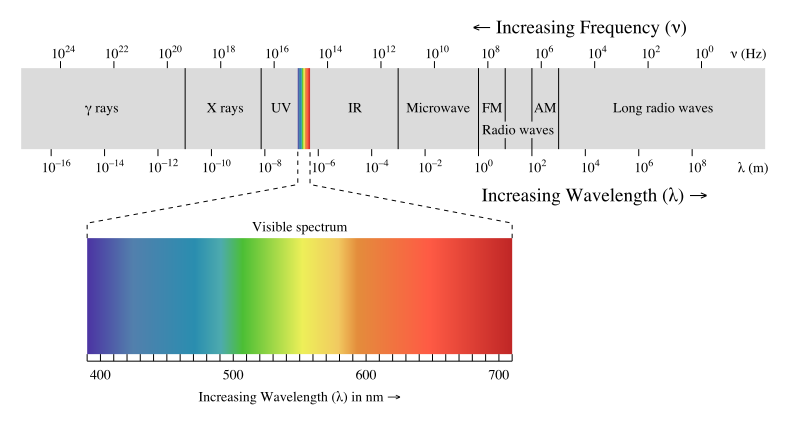
\includegraphics[width=16.866cm,height=9.022cm]{EMRad-img001.png}

https://ru.wikipedia.org/wiki/\%D0\%A4\%D0\%B0\%D0\%B9\%D0\%BB:EM\_spectrum.svg

 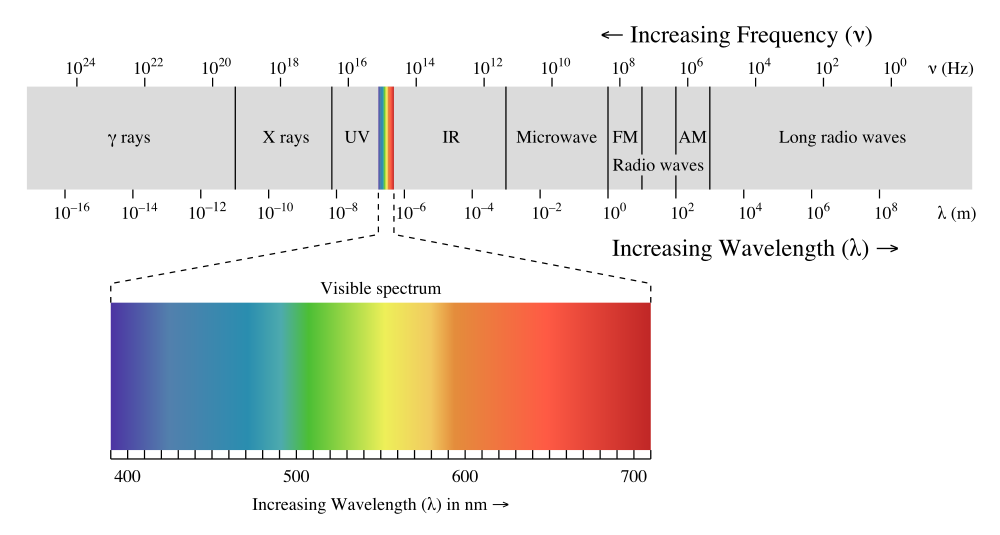
\includegraphics[width=15.665cm,height=8.382cm]{EMRad-img002.png}

 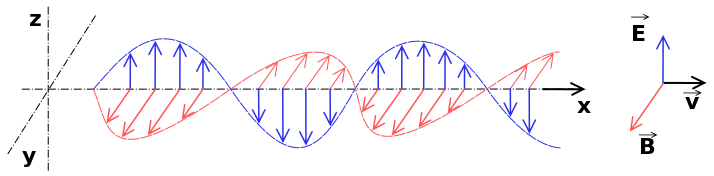
\includegraphics[width=14.713cm,height=3.627cm]{EMRad-img003.png}

http://nuclphys.sinp.msu.ru/introduction/nobelprice.htm


\end{document}



%%%%%%%%%%%%%%%%%%%%%%%%%%%%%%%%%%%%%%%%%%%%%%%%%%%

% Local Variables:
% TeX-parse-self: t
% TeX-auto-save: t
% TeX-master: t
% End:
